%Pavel Chvykov


% ***********************************************************
% ******************* MY HEADER ************************
% ***********************************************************
%\documentclass[11pt]{article}
\documentclass[reprint,prx]{revtex4-1}
%\documentclass[prb]{revtex4-1}
%\documentclass[twocolumn,showpacs,preprintnumbers,amsmath,amssymb,superscriptaddress]{revtex4-1}
%\usepackage[greek, english]{babel}

\usepackage{amsmath} % AMS Math Package
\usepackage{amsthm} % Theorem Formatting
\usepackage{amssymb}	% Math symbols such as \mathbb
\usepackage[pdftex]{graphicx}
\usepackage{epstopdf}
\usepackage{enumerate}
%\usepackage{multicol} % Allows for multiple columns
\usepackage{wrapfig}
\usepackage[dvips,letterpaper,margin=1in,bottom=1in]{geometry}
\usepackage{color}
\usepackage{tensind}
\tensordelimiter{`}
\whenindex{a}{\alpha}{} \whenindex{b}{\beta}{} \whenindex{g}{\gamma}{} \whenindex{d}{\delta}{} \whenindex{e}{\varepsilon}{} \whenindex{m}{\mu}{} \whenindex{n}{\nu}{} \whenindex{l}{\lambda}{} \whenindex{k}{\kappa}{} \whenindex{r}{\rho}{} \whenindex{s}{\sigma}{} \whenindex{t}{\tau}{}
\usepackage{todonotes}
\usepackage{subcaption}
\captionsetup{justification=raggedright,singlelinecheck=false}
%\usepackage{subfig}
% % Sets margins and page size
%\pagestyle{empty} % Removes page numbers
\usepackage{setspace}
%\onehalfspacing
%\setstretch{1.1}
\usepackage{comment}
\usepackage{cancel}
%\usepackage{xfrac}
\usepackage[]{units}

\usepackage{hyperref}
\usepackage[all]{hypcap}
\makeatletter % Need for anything that contains an @ command 

%\renewcommand{\maketitle} % Redefine maketitle to conserve space
%{ \begingroup \vskip 10pt \begin{center} \Large {\bf \@title}
%		\vskip 10pt \large \@author \\ \@date \end{center}
%		\vskip 10pt \endgroup \setcounter{footnote}{0} }


%\makeatother % End of region containing @ commands
%\renewcommand{\labelenumi}{(\alph{enumi})} % Use letters for enumerate
% \DeclareMathOperator{\Sample}{Sample}
\let\vaccent=\v % rename builtin command \v{} to \vaccent{}
\renewcommand{\v}[1]{\ensuremath{\vec{#1}}} % for vectors
\newcommand{\gv}[1]{\ensuremath{\mbox{\boldmath$ #1 $}}} 
% for vectors of Greek letters
\newcommand{\uv}[1]{\ensuremath{\mathbf{\hat{#1}}}} % for unit vector
\newcommand{\abs}[1]{\left| #1 \right|} % for absolute value
\newcommand{\avg}[1]{\left< #1 \right>} % for average
\let\underdot=\d % rename builtin command \d{} to \underdot{}
\renewcommand{\d}[2]{\frac{d #1}{d #2}} % for derivatives
\newcommand{\dd}[2]{\frac{d^2 #1}{d #2^2}} % for double derivatives
\newcommand{\pd}[2]{\frac{\partial #1}{\partial #2}} 
% for partial derivatives
\newcommand{\pdd}[2]{\frac{\partial^2 #1}{\partial #2^2}} 
% for double partial derivatives
\newcommand{\pdc}[3]{\left( \frac{\partial #1}{\partial #2}
\right)_{#3}} % for thermodynamic partial derivatives
\newcommand{\fd}[2]{\frac{\delta #1}{\delta #2}} %functional derivative
\newcommand{\fdd}[3]{\frac{\delta^2 #1}{\delta #2 \delta #3}} %second functional derivative
\newcommand{\ket}[1]{\left| #1 \right>} % for Dirac bras
\newcommand{\bra}[1]{\left< #1 \right|} % for Dirac kets
\newcommand{\braket}[2]{\left< #1 \vphantom{#2} \right|
\left. #2 \vphantom{#1} \right>} % for Dirac brackets
\newcommand{\matrixel}[3]{\left< #1 \vphantom{#2#3} \right|
#2 \left| #3 \vphantom{#1#2} \right>} % for Dirac matrix elements
\newcommand{\grad}{\nabla} % for gradient
\let\divsymb=\div % rename builtin command \div to \divsymb
\renewcommand{\div}[1]{\gv{\nabla} \cdot #1} % for divergence
\newcommand{\curl}[1]{\gv{\nabla} \times #1} % for curl
\newcommand{\tr}{\mbox{tr}}
\let\baraccent=\= % rename builtin command \= to \baraccent
\renewcommand{\=}[1]{\stackrel{#1}{=}} % for putting numbers above =
\renewcommand{\deg}{^{\circ}} %degree simbol
\renewcommand{\(}{\left (}
\renewcommand{\)}{\right  )}
\renewcommand{\[}{\left [}
\renewcommand{\]}{\right ]}
\newcommand{\<}{\left <}
\renewcommand{\>}{\right >}

\newtheorem{prop}{Proposition}
\newtheorem{thm}{Theorem}[section]
\newtheorem{lem}[thm]{Lemma}
\theoremstyle{definition}
\newtheorem{dfn}{Definition}
\theoremstyle{remark}
\newtheorem*{rmk}{Remark}
\newtheorem{?}{\textbf{Question}}

\newcommand{\e}[1]{\mbox{e}^{#1}} %exponential
\renewcommand{\exp}[1]{\mbox{exp}\[#1\]} %exponential
\newcommand{\intmom}[2][4]{\int \frac{d^{#1} #2}{(2\pi)^{#1}}} % 4D momentum integral
\newcommand{\intfn}{\int \mathcal{D}} %functional integral
\newcommand{\D}{\mathcal{D}}
\newcommand{\bigO}[1]{O\(#1\)}  %order of (big O notation)
\newcommand{\Op}{\mathcal{O}}  %operator
\newcommand{\im}{i}  %imaginary
\renewcommand{\Im}{\mbox{Im}}  %imaginary
\renewcommand{\Re}{\mbox{Re}}  %imaginary
\renewcommand{\todo}[1]{\textit{\color{red}[#1]}}
\newcommand{\um}{$ \mathrm{\mu} $m}
\renewcommand{\inf}{\infty}
\newcommand{\with}{\quad \text{with} \quad}
% ***********************************************************
% ********************** END HEADER *************************
% ***********************************************************

\begin{document}
		\title{Least Rattling in Smarticles}
		
		\author{author list} %\thanks{pchvykov@mit.edu}
		
		\maketitle


\tableofcontents

%\begin{itemize}
%	\item Introduction
%	\item regularization in smarticles
%	\item Effective noise Teff, correlation
%	\item Other configurations: random, phase-offset
%	\item breaking this - inertial (do exp't with less inertia?)
%	\item RWRM -- graph and diffusion
%	\subitem as max-caliber
%	\item Discussion
%\end{itemize}

\section{Introduction}
A common intuition is that it is much easier to get a collection of many particles to move in a disorderly way than in an orderly one. To found this idea more rigorously, one may invoke the idea of molecular chaos, which supposes that simple, non-linear pair forces acting amongst many colliding particles will lead to quasi-random motion. By definition, specific patterns of order in structure or dynamics are extremely rare compared with the vast array of alternative states or trajectories for the system, and when fluctuations from molecular chaos are uniform across a whole configuration space, order is disfavored in proportion to this rarity.  

Once the strength of fluctuations is allowed to vary across space, however, it is clear even in simple systems that random motion can itself be the cause of low-entropy ordering.  A one-dimensional Fokker-Planck equation with a spatially-varying diffusion coefficient yields a steady-state probably distribution shaped like p(x)~1/D(x), which means one may favor one location in space over all others simply by making the stochastic noise much weaker there.  Indeed the transport of Brownian particles by thermophoresis is thought to operate by this mechanism, and in such cases, the spatial variation of noise is imposed externally through the creation of a thermal gradient. In many-body systems driven by time-varying forces, however, molecular chaos allows for inhomogeneity of fluctuations across configuration space to be an emergent property of how the internal dynamical rules combine with the particular pattern of driving.  Such scenarios abound in active matter, pointing to the possibility of understanding spontaneous order in these systems by investigating fluctuations.

Active matter can be described as a diverse class of externally-driven many-particle systems that are fed by energy sources distributed over many microscopic degrees of freedom. Active matter systems have recently attracted intense interest from both experimenters and theorists, particularly as more examples have been discovered where an inverse cascade of energy from microscopic to macroscopic scales gives rise to complex ordered structures and system-scale dynamical patterns. Self-propelled colloidal particles, for example, have been shown to assemble into highly dynamic “living crystal” structures [44], while motor-driven protein filaments were observed to form large-scale spiral whorls and topological defects [50, 27]. With the advent of swarm robotics, it has also become possible to study active matter experimentally with a greater degree of control and detail….


\section{Smarticles}
We conducted our experiments with a collection of small simple robots called ``Smarticles'' (smart active particles) (fig. \ref{fig:smarticle}). Each one is comprised of three connected links, with the two hinges being controlled by a programmable micro-controller via stepper motors. When the Smarticle is sitting on its base, the arms do not touch the ground, and so an individual smarticle cannot move. A group of them, on the other hand, can achieve complex motion by pushing off each other. Here we will focus on the regime where their arms are executing a periodic motion pattern, which we call ``gait,'' with no feedback from the environment (note that the gait timing is kept by the controller, and hence the cycle's phase is not affected by forces on the arms). Such gaits can be represented (uniquely up to rate) as closed loops in the two-dimensional conformation space (the two hinge angles) of the Smarticle (fig. \ref{fig:smarticle}). In the first part of the paper, we will have all Smarticles execute a synchronized ``square'' gait (fig. \ref{fig:smarticle}). \todo{Include all the technical details of realization and construction of Smarticles and synchronization in an appendix?}

The whole setup placed on an aluminum plate leveled to $ < 0.1\deg $. The ring is 19.2 cm in diameter, and is glued to the plate below such that it cannot move or deform. The smarticles perform a square gait locked in phase with each other.

\begin{figure} 
	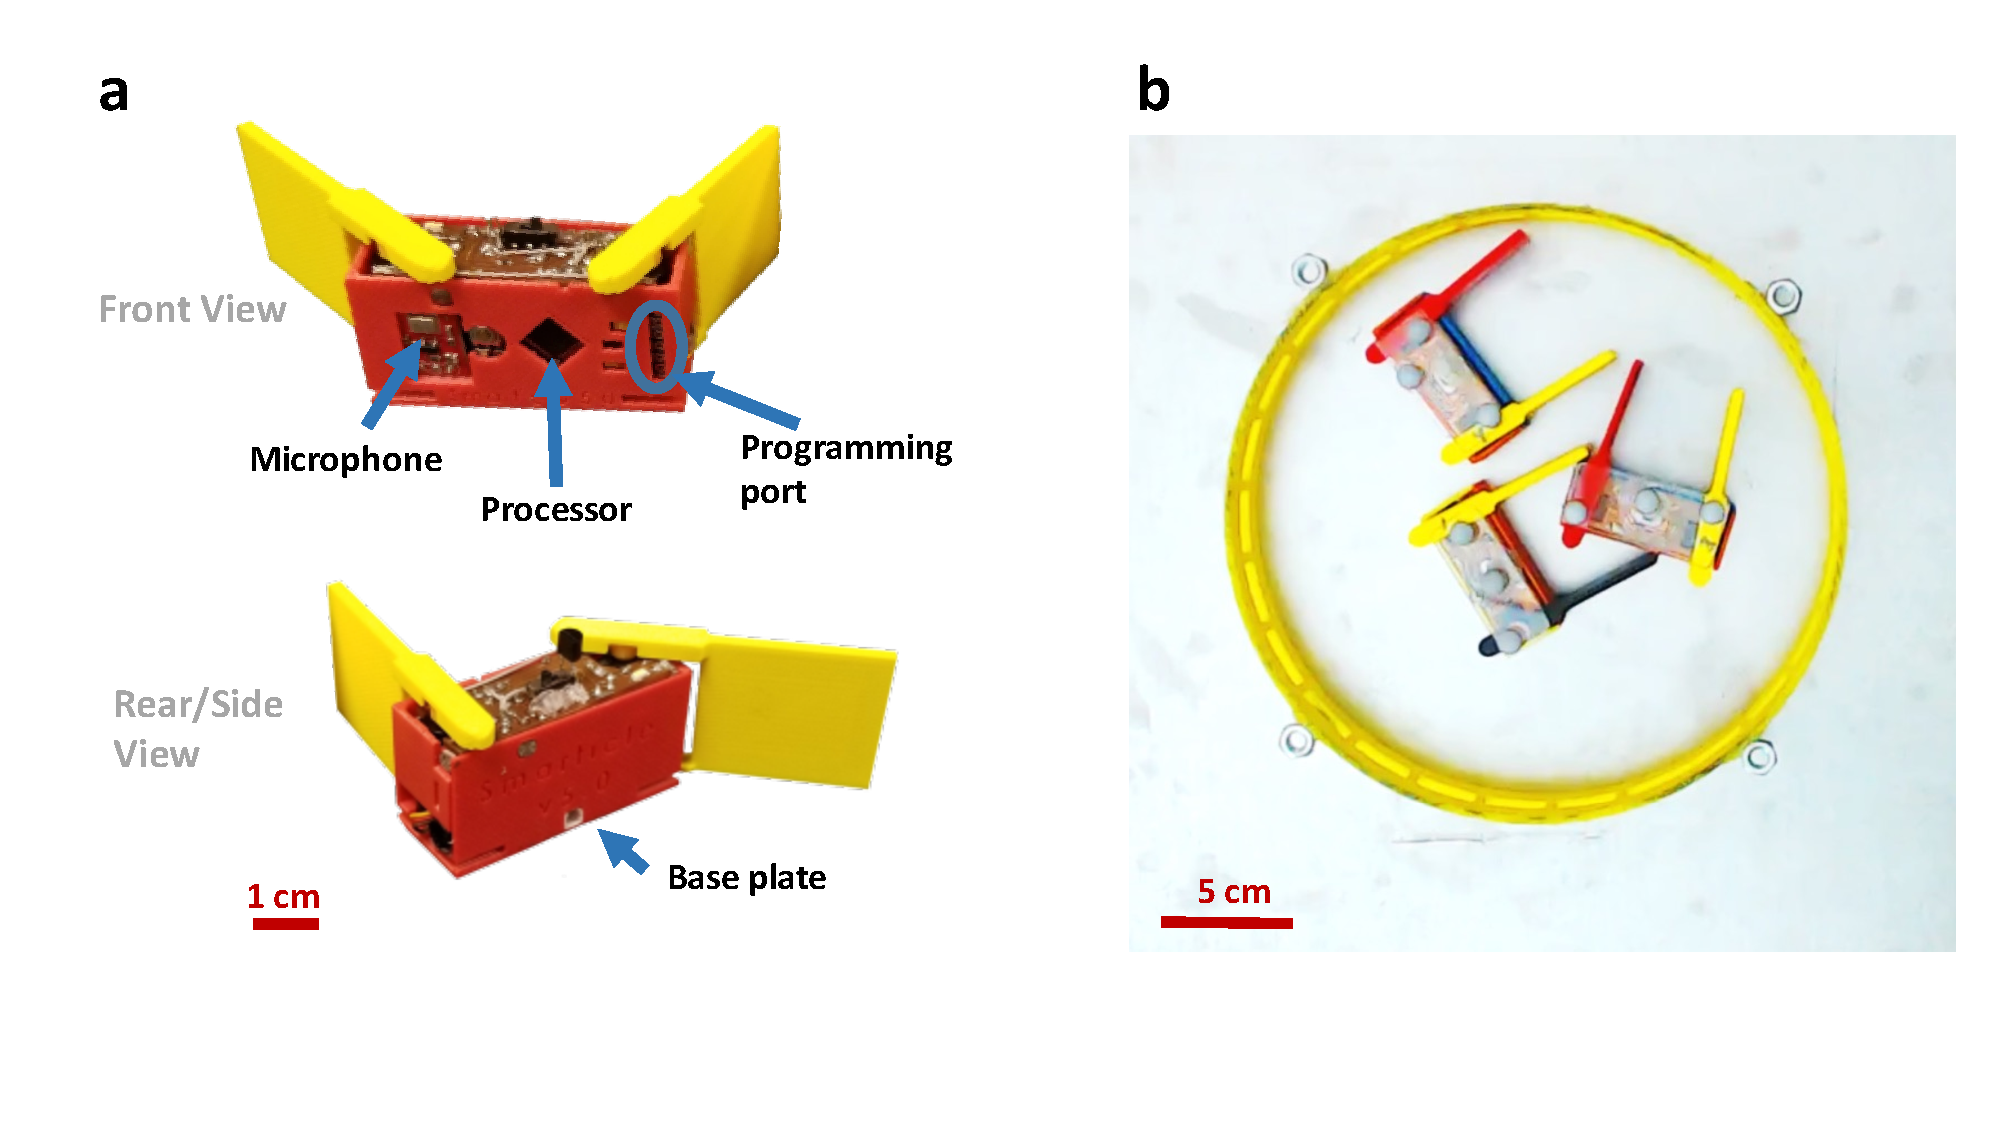
\includegraphics[width=0.5\textwidth]{expt.pdf}
	\caption{a) Diagram of a single Smarticle robot. b) One simple setup to look for collective self-organizing dynamics (view from above).}
	\label{fig:smarticle}
\end{figure}

We place three Smarticles on a flat aluminium plate, inside a glued-down plastic ring (fig. \ref{fig:super3}). By moving their arms, the robots can push off each other, while the ring prevents them from decoupling -- thus forming an optimal play-ground to look for dynamical emergence. To get data, we use Optitrack \todo{details} to track the full time-evolution of the 2D coordinates and body-angle $ (x,y,\theta) $ of each robot at 120 frames per second (we do not track the arm positions). 

For experiment prototyping and better sampling statistics, we have also built a simulation of this setup, described in Appendix \ref{app:simulation}, and benchmarked it against experiments. Both experimental and simulation data are then fed through a pre-processing pipe-line, which mods out the rotation and permutation symmetries of the 3-Smarticle setup, thus reducing the effective configuration space substantially (Appendix \ref{app:dataAnal}).



\section{Regularization}

\begin{figure*}
	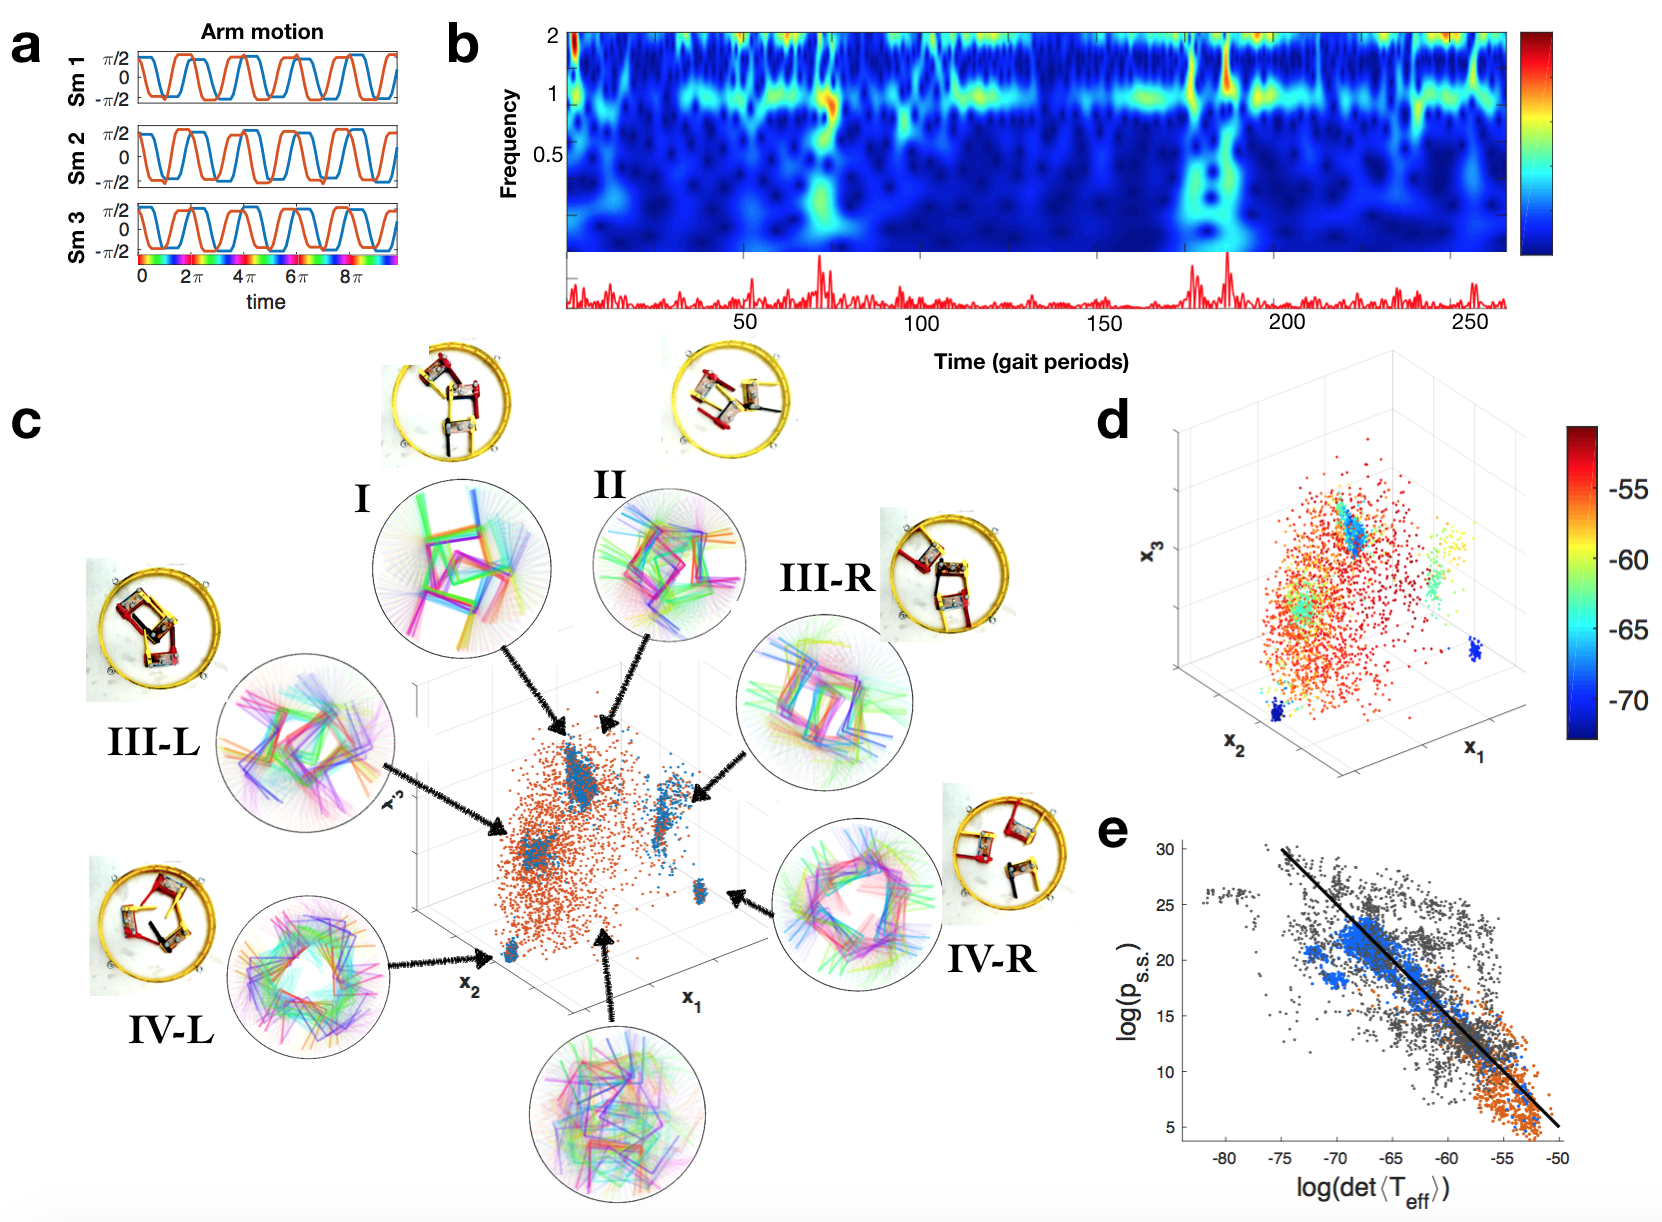
\includegraphics[width=1\textwidth]{3regularization.png}
	\caption{a) Synchronized ``square gait'' arm motion pattern of the three smarticles; b) Wavelet transform of one Smarticle's x-coordinate over a 10-min experimental run. Broad-band amplitude plotted below indicates how organized the dynamics are at different times. c) Dynamical regular states that emerge in this setup: initial conditions for each [exp't]; time evolution along the color-axis (as labeled in (a)) for 3 gait periods [sim]; system position in its configuration space (stroboscopic, projected to 3D) - blue points sampled from long-time evolution, red sampled by randomly dropping smarticles in the ring [sim] -- illustrating the spontaneous fine-tuning (note: states I and II are indistinguishable in this projection; states III and IV have two chiral compliments). d) Configuration space points colored by $\log(\det \<T_{eff}\>)$ of their neighborhood [sim] -- long trajectories spend most of their time in low-$T_{eff}$ regions. e) correlation illustrating steady-state probability $p_{s.s.} \propto 1/\det \<T_{eff}\>$ (black line): experimental data for long trajectories is in grey, simulation data is in blue/red (for different regions of configuration space, as in (c))}.
	\label{fig:reg}
\end{figure*}

In general, the response properties of a dynamical system to an external drive will depend on the system's configuration. In particular, a given drive can cause chaotic motion in some parts of the configuration space, while being perfectly organized elsewhere. To check if this applies here, we set all three Smarticles to execute a phase-synchronized square gait inside a glued-down ring, track the trajectories, and plot out the wavelet transform of the orientation of any one Smarticle -- fig. \ref{fig:wavelet}. As the energy from the drive is injected at a particular frequency, we always see a peak in the power-spectrum there. On the other hand, the amount to which that energy gets dispersed to other frequencies before dissipating out varies as the system explores different configurations over time. In the regions where a large broad-band component emerges, we have very noisy dynamics. The lack of a broad-band component, on the other hand, indicates that the dynamics are orderly, which we may be surprised to find in such a messy system. 

%While there is always a peak in the power-spectrum at the driving frequency, the broad-band amplitude (particularly obvious in lower frequencies) clearly changes over time. As broad-band of the power-spectrum accounts for the disordered component of the motion, this illustrates that dynamics go through periods with more or less effective noise. 
%When all the Smarticles are executing a phase-synchronized square gait,
Taking a closer look at these regular dynamics, we see that there the three Smarticles organize into one of several periodic dynamical patterns (a sort of collective organized dance) \todo{videos in supplement}. Figure \ref{fig:configSpace} gives some illustration of the fine-tuning associated with this \todo{better visualization of regular states???}. Such self-organization is perplexing, and its interpretation depends on the perspective we take -- that of dynamical systems theory, or thermodynamics.
\todo{not synchronization}



From the context of dynamical systems, perhaps it is not surprising that the dynamics of a time-periodic system are governed by several limit-cycle attractors. On the other hand, not all periodic systems relax to such attractors -- even here we can make slight changes to our setup, such as changing relative gait phases, or making Smarticles inertial \todo{figures for this here?}, so as to make the system behave chaotically. Furthermore, this system cannot really be seen as deterministic, as we know that it is strongly affected by the stochasticity coming from the hard-boundary interactions between non-smooth shapes, and highly surface-sensitive effects of sliding friction.

From the perspective of equilibrium thermodynamics, where entropy and disorder tend to a maximum, this sort of self-organization may seem extremely surprising. Of course, this system is far from equilibrium, and so entropy need not grow. Indeed, for a Brownian particle diffusing in a compact domain of inhomogeneous temperature $ T(\v{x}) $ (and no other forces), we know that the steady-state probability distribution will be $ p_{s.s.} \propto 1/T(\v{x}) $ -- which can be far from the maximum-entropy uniform distribution. We want to use this example to motivate our explanation of the fine-tuning we observe.

Indeed, the intuition is the same: probability concentrates in regular states, which are, in some sense, less noisy than the chaotic behavior in other parts of the configuration space. We can make this intuition precise by defining an effective temperature $ T_{eff}(\v{x}) $ at every point in the configuration space, and checking if it correlates with $ p_{s.s.}(\v{x}) $. While this system is too complicated to calculate $ T_{eff} (\v{x})$ from first principles, we can ``measure'' it numerically from ensembles of short trajectories starting at $ \v{x} $. Our hypothesis, therefore, is that we can predict the long-term behavior from looking only at short trajectories -- which need not be possible for far-from-equilibrium systems. 

%While we could try to go into a mechanistic explanation for the self-organization in our setup, it would likely be very specific to the parameters and choices used here and would not generalize well to other configurations of Smarticles, or to other active matter systems. Instead, we want to give a less fundamental, but more generalizable explanation. We note that for most initial configurations of the three Smarticles in a ring, after one period of arm motion they go to a new configuration. For some specific configurations, however, they stay in the same place -- and these are precisely the periodic limit-cycle attractors we see in any long trajectory (fig. \ref{fig:configSpace}). This may at first seem tautological: at long times the system tends to be found in places from where it does not leave. The rest of the paper will be explaining why this is both, highly non-trivial in a precise mathematical sense, and also profound for understanding real-world strongly-driven systems \todo{references to sections}. 

\section{Defining $ T_{eff} $}
The question, therefore, is how can we extract a measure of effective noise amplitude from looking at short trajectories. On one hand this system is periodic in time, so one natural metric would be to look at the distance it moves in configuration space over one period. Another natural metric could be inspired by Brownian dynamics $ \dot{x}=\sqrt{2\;T(x)}\cdot\xi $, and so \todo{T inference }$ T(x)=\int dt\;\<\dot{x}(t)\;\dot{x}(0)\>/2 $, or in higher dimension, we can take the trace of the correlator $ T(x)=\sum_i\<\dot{x}_i\;\dot{x}_i\>/2 $ (see Appendix \ref{app:defRatt} for details). 
We then color the points in fig. \ref{fig:configSpace} by this $ T_{eff} $, and see that the regions of low $ T_{eff} $ correspond precisely to the concentration of steady-state probability. More precisely, fig. \todo{fig:corr} shows the scatter plot of $ p_{s.s.}(x) $ vs. $ T_{eff}(x) $, showing the correlation.

Note that this may at first seem tautological: at long times the system tends to be found in places from where it does not leave. However, below we will explain why this is both, highly non-trivial in a precise mathematical sense, and also profound for understanding real-world strongly-driven systems 
\begin{figure}
	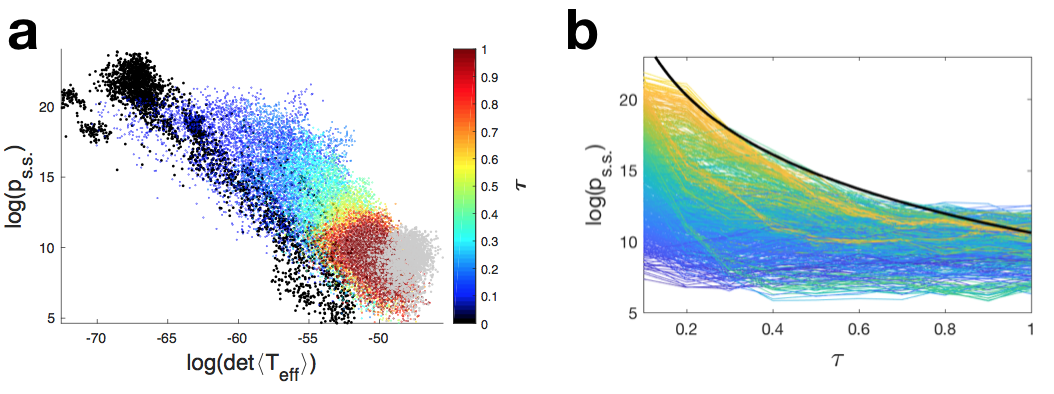
\includegraphics[width=0.5\textwidth]{inertial.png}
	\caption{Destroying regularization by reducing Smarticle damping. a) The overdamped run (black points, from fig. \ref{fig:reg}e) is predictive of all simulations with lower damping (color = velocity decay time-scale $ \tau $), which fall along the same line; light grey -- experimental data for weakly-damped Smarticles. b) Effect of damping on $ p_{s.s.} $ at 1000 different points in configuration space [sim] (color by plot's left edge); black curve is a theoretical prediction for the upper edge (with one fitting parameter).}
	\label{fig:inertial}
\end{figure}
Colored points lie along the black ones, indicating that $T_{eff}$ is predictive of $p_{s.s.}$, whether the noise comes from inertia or from chaotic interactions \todo{universality}.
 

\section{Drive-specificity}
Why should a driven dynamical system get an inhomogeneous $ T_{eff}(x) $ landscape? For a given form of the drive signal, different system configurations will have a different response. In particular, some configurations will respond in a more predictable way than others. In our Smarticle setup, for some initial conditions the sources of stochasticity (such as corner collisions) will be more prevalent than elsewhere. This way, a system settles into drive-specific configurations that give more orderly and stable response properties, and changing the drive will change these selected states. For Smarticles, this would imply that the regular states found at long times are specific to the gait, which is confirmed in experiments (fig. \todo{different gait reg states}). To illustrate that our approach generalizes beyond periodically-driven systems, we can even make the gait random in time, though identical across Smarticles to allow diversity of response properties \todo{figure}.

Another prediction we can make from our framework is that raising the apparent noise uniformly for all configurations $ T_{eff}(\v{x}) \rightarrow T_{eff}(\v{x})+T_0$ will effectively level the steady-state distribution for a large enough $ T_0 $, and thus break the regularization we observe. Experimentally we can realize this by putting smarticles on top of a bed of small, light beads (fig. \todo{smarticles on beads}), thus effectively reducing the friction between Smarticles and the table. This makes every interaction have a larger and less predictable effect, which affects all states in a very similar manner.

\todo{Random correlated arms}\\
\todo{example with more Smarticles}\\
\todo{inertial smarticles}\\
\todo{drive-specificity: change drive only and show T(x) change}
%This results in certain configurations being selected by any given drive as having a lower effective noise, and thus becoming attractive. We can illustrate this intuition by changing the gait in our Smarticle system, and seeing new configurations becoming attractive. 
\begin{figure}
	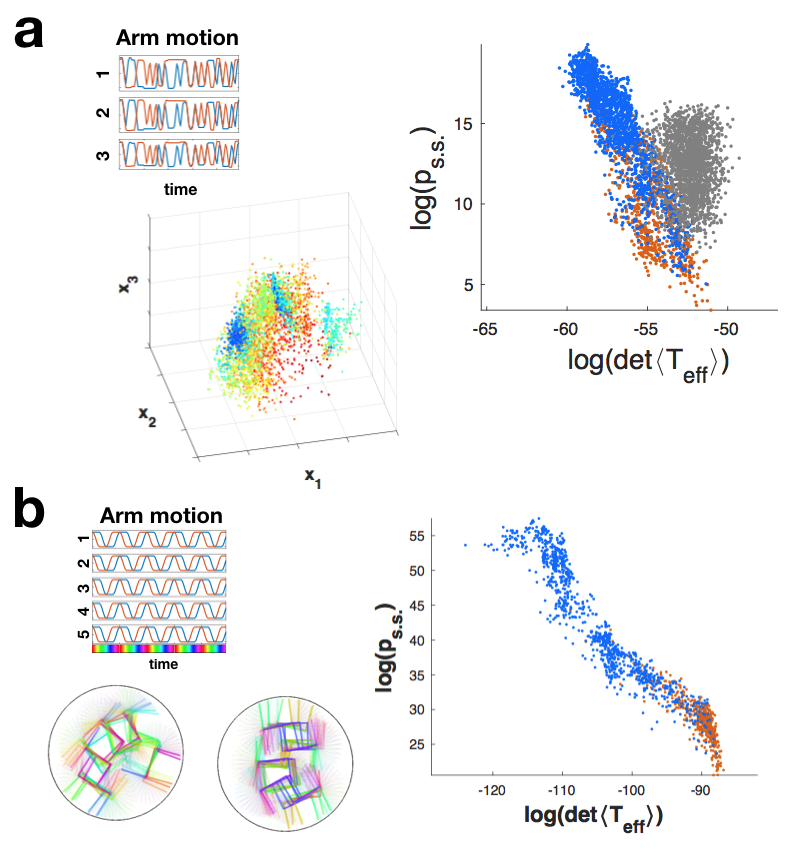
\includegraphics[width=0.5\textwidth]{otherRuns.png}
	\caption{a) A-periodic drive: arms move in a random, but synchronized fashion. $ T_{eff} $ distribution is different from fig.\ref{fig:reg}d -- different regular states emerge. $ p_{s.s.} $ is still strongly correlated with $ T_{eff} $, though the exponent is no longer -1. Grey -- random and independent arm motion, leaving no structure in the drive for adaptation. b) 5 Smarticle group executing synchronized square gait shown similarly produces fine-tuned regular states (two sample ones are shown). Note that most of the red points in the scatter plot are confined to high-$ T_{eff} $ region, indicating a higher degree of fine-tuning in regular states than for 3 Smarticles. [all data from simulation].
		%that regular states occupy an even smaller volume in configuration space than for random initial conditions almost never fall near regular states.
	}
	\label{fig:otherRun}
\end{figure}

\section{Broader impact}
Our $ T_{eff}(\v{x}) $ is effectively a measure of instability of the configuration $ \v{x} $. Hence, a statement that at steady-state the systems tends to be found in configurations that are more stable (in places it does not leave) may seem tautological at first. However, the key here is that this measure is local -- depends only on the state $ \v{x} $ itself, and not on the rest of the landscape. Landauer's ``blowtorch theorem,'' \todo{cite} on the other hand, shows that for general nonequilibrium systems, the value of the steady-state probability at a point $ \v{x} $ can depend on system properties at any arbitrarily far-away points. Hence having any local quantity that is predictive of the $ p_{s.s.} $ is highly non-trivial and is indicative of additional structure in the system. It can, in some sense, be seen as a generalization of equilibrium thermodynamics -- there, detailed balance ensures that the steady-state is determined locally. In our case, on the other hand, we try to leverage the additional assumption of ``complexity'': we think of our system as so complex, high-dimensional, and ``generic'' that it can essentially be approximated as random. We argue that this is really the ``typical'' scenario -- while it can be violated, such a violation would require fine-tuning, which becomes progressively less likely in more complex high-dimensional systems.

\begin{figure}
	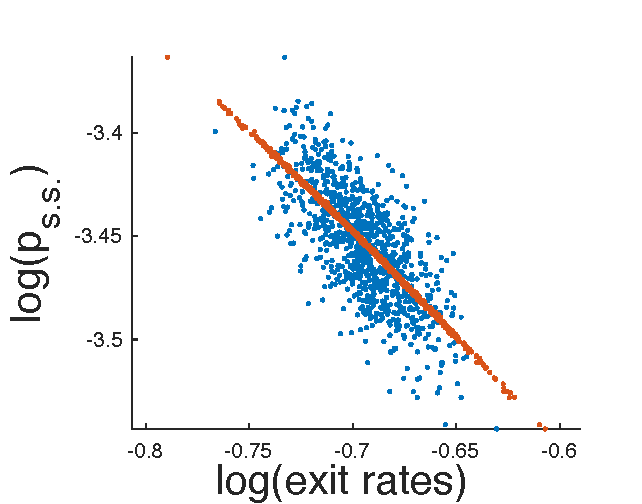
\includegraphics[width=0.55\textwidth]{randMark.pdf}
	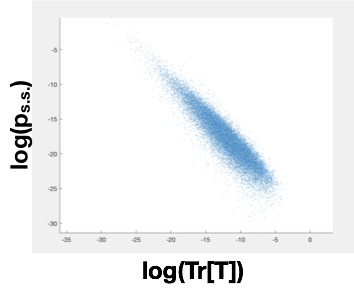
\includegraphics[width=0.45\textwidth]{randDiff.png}
	\caption{a. Steady state for a Markov process with $ 1000 \times 1000 $ random transition matrix. Blue points show exit rates, red points also include the correction from entrance rates.
		%Blue points show $ \frac{\bar{R}}{\sum_j R_{ij}} $, which depends only on the exit rates, and red points also include the correction due to the entrance rates $ +\frac{\sigma}{\bar{R}\,N^{3/2}}\, \xi_i $ 
	b. Steady state vs. trace of temperature tensor for multivariate inhomogeneous diffusion in a random temperature landscape}
	\label{fig:randDynamics}
\end{figure}

There are several ways to make this discussion more precise. One way to look at it is to consider a Markov process $ \dot{p}_i= \sum_j R_{ji}\, p_j - \sum_j R_{ij}\, p_i $, with $ N $ states $ i\in\{1,...,N\} $. In general the steady-state distribution $ p_{s.s.}(i) $ will depend on all the $ N^2 $ transition rates. Now, if we let the transition rates $ R_{ij} $ to be independent identically distributed random variables (with some mean $ \bar{R} $ and standard deviation $ \sigma $), and let $ N \rightarrow \infty$, then it is easy to show \todo{Appx or citation} that $ p_{s.s.}(i)= \frac{1}{N} + \sum_j (R_{ji} - R_{ij})/(N^2\,\bar{R}) + \bigO{N^{-3}}$. The first term $ \sum_j R_{ji} $ is the total entrance rate into state $ i $, and may in a real system be hard to measure, as it would require initializing the system in all possible configurations and seeing how often it enters $ i $. The second term $ \sum_j R_{ij} $, on the other hand, is the total exit rate, and is akin to our measure of $ T_{eff} $ -- it is basically a measure of how stable the state $ i $ is and only requires local measurements initialized in that state. We can rewrite the expression for the steady-state focusing on the exit rates: $ p_{s.s.}(i)= \frac{\bar{R}}{\sum_j R_{ij}} + \frac{\sigma}{\bar{R}\,N^{3/2}}\, \xi_i$, where $ \xi_i \equiv  \sum_j \(R_{ji}-\bar{R}\)/\(\sigma\,\sqrt{N}\)\sim 
\mathcal{N}[0,1]$ -- univariate Gaussian random variable (note however that it is correlated with $ p_{s.s.}(i) $). So while in general we need all $ N^2 $ rates to predict the steady-state, the randomness in rates allows us to express it in terms of just $ N $ local measurements of the exit rates, up to a noise term from  the unobserved entrance rates \ref{fig:randDynamics}a.
%This simple model thus qualitatively reproduces what we observe in the Smarticle system: that exit rate is predictive of the steady-state density, albeit not perfectly because of the additional influence of the entrance rates 

It turns out we can make an even stronger statement if we consider the $ d $-dimensional diffusion process on a compact domain $ \dot{x}_i = D_{ij}(x)\cdot\xi_j $ [Ito], $ i\in\{1,...,d\} $, $ \v{x}\in\mathbb{D}^d $, where the diffusion tensor $ D_{ij} $ varies smoothly over $ x $, but is otherwise random. Again, as this is a non-equilibrium process, in general the steady-state density at any point will depend globally on the diffusion tensor everywhere: $ p_{s.s.}(x) = f_x\[D_{ij}(y)\; |\; y\in \mathbb{D}^d \]$. However, the random choice of $ D_{ij}(x) $ simplifies this result: we can numerically show that $ p_{s.s.}(x) \sim 1/\tr\(T(x)\) $ for $ T \equiv D\, D^T$ \ref{fig:randDynamics}b, as long as the variation of $ \tr\(T(x)\) $ is sufficiently large. 

Finally, we can also frame our results in a somewhat different light. 
Thus, while the exact dynamics generally give a complicated $ p_{s.s.}(x) $, we can view $1/T_{eff}(x) $ as the least-informative approximation based on only local information.
We think of approximating the system behavior by ``typical'' dynamics that match the local fluctuation amplitude of the system $ T_{eff}(x) $. Concretely, we find the maximum-entropy (or ``max-caliber'' \cite{dill18max_caliber}) probability distribution over trajectories $ P[\v{x}(t)] $, constraining the local velocity fluctuations: maximize 
\begin{align*}
\mathcal{S} = P[x] \;\log\(P[x]\) + \lambda_0 \( \int \mathcal{D} x \;P[x] - 1\) + \\
\int dX \; \lambda(X) \(\sum _i \< \dot{x}_i\,\dot{x}_i\> _X - T_{eff}(X)\)
\end{align*}, where $ \< \dot{x}_i\, \dot{x}_i\> _X \equiv \int \mathcal{D}x \; P[x] \,\int dt \; \dot{x}_i(t) \dot{x}_i(t) \,\delta(x(t) - X) $. This gives $ P[x(t)] \propto \exp{-\sum_i \int dt \; \lambda(x(t))\,\dot{x}_i(t)\dot{x}_i(t)} $, which corresponds \todo{uniquely} to the stochastic process $ \dot{x}_i = \sqrt{2\,T_{eff}(x)}\cdot \xi_i$, whose steady-state distribution is $ p_{s.s.}(x)\propto 1/T_{eff}(x) $. \todo{explain this paragraph better - too dense, and interesting}


\todo{coordinate dependence}

%In a sense, we found here a local observable that is predictive of the steady-state density in a complex far-from-equilibrium system. This is surprising -- indeed, Landauer showed \todo{cite blowtorch} that for general nonequilibrium systems, the value of the steady-state probability at a point $ \v{x} $ can depend on system properties at any arbitrarily far-away points -- and hence no local observable can exist that predicts $ p_{s.s.}(\v{x}) $. With additional assumptions however, this can become possible -- e.g., the assumption of detailed balance gives the Boltzmann distribution, which depends only on the local energy (up to normalization). Here, we try to leverage the additional assumption of ``complexity'' -- we think of our system as so complex, high-dimensional, and ``generic'' that it can essentially be approximated as random.








\appendix
\renewcommand{\thesection}{\Alph{section}} 
\section{Experiment details} \label{app:experiment}

Most of the Smarticle design and experiment setup details are described in a previous publication \todo{cite once out}. The key difference from the experiments in that work is that here the gaits of the different smarticles in the ensemble were kept synchronized throughout the runs, which is what allowed them to fall into regular dynamical patterns not previously observed. This synchronization was achieved by connecting a microphone sensor to an interrupt pin of the micro-controller in each smarticle, and then triggering every gait with a beep from external speaker placed next to the setup. This meant that all the smarticles stopped momentarily between consecutive gaits to listen for the trigger -- but this stop was kept down to a fraction of a second by carefully timing the triggering pulse-train with the gait period. The resulting setup was robust enough to keep the experiment running and synchronized indefinitely (limited only by battery life to about 1 hour). It also ensured that the arm motion was precisely periodic throughout the experiment, with no possibility for any phase drifts of fluctuations.  

Another minor difference is that for the experiments presented in this work, the boundary ring was glued down for simplicity. Also, as mentioned, here we ran experiments with just 3 identical smarticles, rather than the more intricate setups of that paper. 


\section{Simulation details} \label{app:simulation}
For easier exploration of hypothesis space of this system, we have constructed a numerical simulation with the following algorithm. We approximate smarticles by three-segment lines (insets in fig. \ref{fig:dimRedSim}). At each time-step, the algorithm moves the arms slightly according to the chosen gait, and then iteratively cycles through smarticle pairs in random order, checking for collisions, and moving one in each pair slightly according to the net interaction force. If there are multiple points of contact for a given pair, the move is a translation in the direction of the total force, otherwise, it is a rotation about a pivot point chosen so as to balance the forces and torques. Choosing which in the pair moves is random, weighted by their relative friction coefficients (as motivated by difficulty of predicting static friction). Note that since a move can create new collisions with other smarticles, it is important to take small steps and iterate. The algorithm continues looping through pairs until all collisions are resolved, then proceeding to the next time-step. While this describes the core of the algorithm, there are a number of bells and whistles necessary to improve its stability and reliability:
\begin{itemize}
	\item  If two arms are near-parallel when they approach each other, they can pass through each other between ticks without ever intersecting. To prevent this, along with collision detection, we must explicitly test for this in each pair. We then store the order of the arms for a few ticks into the future to prevent them passing through each other in any of those times.
	\item In case a smarticle with small friction gets trapped between two others, it might rattle back and forth on each iteration of collision-resolution, with no net effect. To prevent this, we temporarily (until next tick) increase its friction each time a smarticle moves.
	\item In experiment, when resolving collision is too hard, the motor simply does not move (jams up). To allow for that possibility in simulation, we add an exit condition from the collision-resolving loop for when any one smarticle's temporary friction (from last bullet) becomes very large - as this serves as a proxy for how much force a motor must provide. We then move the most colliding arm back to its last time-step, and try collision-resolving again. If everything resolves, that arm will then have a chance to catch up to where it needed to be over the following ticks (its speed being capped at some $ \omega_{max} $).
	\item The resulting simulation turns out to be too clean, despite the multiple stochastic elements of the algorithm, and so dynamical phases much more stable than in experiments. Since we want to study transition statistics, we must find ways to destabilize them. There are a number of places we can add more noise: slight fluctuations of smarticles' positions and angles at each tick, or proportional to each move, randomly varying gait amplitude, varying arm velocity, etc. Adding inertia or inter-Smarticle friction forces (see below) also helps to destabilize the dynamics.
	\item The ring boundary is implemented similar to other smarticles, and collisions with it are resolved in the same loop. Alternatively, we can implement weakly confining potential to keep smarticles together in a more smooth way (for different experiments).
	\item It is easy to adjust the simulation to give the Smarticle inertia: at each tick, simply move them according to last step's velocity before resolving collisions.
	\item  If inter-Smarticle friction is 0, then each interaction force is directed normal to one Smarticle's surface. To include effects of such friction, we can add a small lateral component to these forces that depends on the interaction angle.  
%	we can also approximate the influence of inter-Smarticle friction by turning the interaction force from the surface normal slightly.
\end{itemize}

Even with all these additions, many differences remain between simulation and experiment: smarticles have non-zero thickness in experiments, there are relief features on smarticle body not present in simulation that can get caught, the precise force-response profile of the motors is not captured, etc. The consequence in this system is that while qualitative features can be recovered in the simulation, we don't generally expect precise quantitative agreement. We guess that these differences may be less important for ensembles with more smarticles -- as universal collective properties start to dominate. We also guess that analytical predictive power of least-rattling, or other similar techniques, could be more applicable in that regime.

\section{Data analysis} \label{app:dataAnal}

Once we have the tracked coordinates of the smarticles over time, either in experiment or simulation, we want to map the data into a ``collective behavior space'' -- something that can usefully inform us about the unique dynamical patterns of motion, which is what we ultimately care about. We can then look at the statistics of steady-state distributions in this space to make the figures shown above. 

The entire configuration space of this system, which then uniquely determines the future dynamics (up to noise), consists of the 2D coordinates and orientations $ (x,y,\theta) $ of all the $ N $ Smarticles in the ensemble, as well as their arm angles $ (\alpha_1, \alpha_2) $. However, this $ 5N $-dimensional space has more information than we minimally need to determine next gait's collective behavior. 

\subsection{Removing configurational symmetries}
First, for all the experiments presented in this work, future arm motion is independent of all the other variables, and is uniquely (or statistically, for the random arm motion) determined by their current state. So the Smarticle coordinates $ (x,y,\theta) $ taken stroboscopically at times when $ (\alpha_1, \alpha_2) = (pi/2,pi/2)$ (U-shape, for all Smarticles) are sufficient to fully determine the future dynamical behavior. Note that this is harder to do precisely in experiment than in simulation, as we cannot track the arms directly, and so must make do with inferring the stroboscopic time-points from motion pattern of the bodies and the knowledge that arms are synchronized and exactly periodic for the entire run. 

Second, because the confining ring is round, the system has a global rotation symmetry -- dynamical patterns that differ only by a global rotation should be counted as the same. To remove this unnecessary information from our data, the easiest way is to use only rotationally-symmetric observables. We can construct these from the $ 3N $-variables we have for each time-point by taking the coordinates of the c.o.m. $ \vec{X}= \frac{1}{3} \sum_i \vec{x}_i $ in the reference frame of each smarticle: $ \vec{\chi}_i \equiv \mathcal{R}(\theta_i) \cdot (\vec{X} - \vec{x}_i) $, where $ \mathcal{R}(\theta_i) $ is the rotation matrix for $ i $-th smarticle orientation (fig \ref{fig:relDat}). Note that this change of variables reduces the dimensionality of our configuration space down to $ 2N $ -- i.e., we lost much more information than just the global rotation. In particular, these new coordinates are entirely invariant under c.o.m. translations relative to the ring, which is relevant -- but we can assume it to be small for a confined system. Additionally, in these coordinates, a smarticle orientation matters more the further it is from c.o.m. -- but again, we can assume that their distance to c.o.m. stays relatively constant. More abstractly, we can get away with such imperfect choice because the errors caused by it are still small compared to the inherent noise in this system. 

Finally third, we must remove Smarticle-permutation symmetry, since in these experiments all the Smarticles are treated as identical. As for rotation symmetry, we do this by changing variables to ones that are inherently permutation-invariant: the first three moments of the distribution of the three $ \{\chi_i\} $ at any fixed time. In order for these variables to have similar sensitivity to changes in raw data, it helps to ensure that they have the same units -- by raising them to the appropriate fractional powers. I.e., $ \mu_1 = \frac{1}{3} \sum_i \chi_i $, $ \mu_2 = \sqrt{\frac{1}{3} \sum_i (\chi_i-\mu_1)^2} $, $ \mu_3 = \sqrt[3]{\frac{1}{3} \sum_i (\chi_i-\mu_1)^3} $ (fig. \ref{fig:piDat}), etc.

In the experiments presented here, we can track the 2D coordinates and orientations $ (x,y,\theta) $ of all the Smarticles in the ensemble (fig. \ref{fig:crdDat}) the entire configuration-space coordinates 

For the experiments presented in this work, however, the raw data can directly give us On the other hand, the 2D coordinates and orientations $ (x,y,\theta) $ of all Smarticles at the start of a gait uniquely (up to noise) determine the ensemble's future evolution -- and we can thus assume a one-ot-one correspondence between the $ 3\,N $-dimensional configuration space (for an $ N $ Smarticle ensemble)


we want to map the data into a ``collective behavior space'' -- something that can usefully inform us about the dynamical patterns of motion, especially those relevant for slow time-scales. This behavior space will typically be very high-dimensional, and to work with it we try to either cluster the data into different discrete behaviors (or dynamical phases), or perform a dimensionality-reduction to embed the data in a 2 or 3 dimensional space we can visualize (and could subsequently cluster if desired). In either case, what we care about is not the location of points in behavior space (which would be arbitrary anyway), but only about the distances between them -- i.e., some measures of similarity of different behaviors. 

The raw data from particle tracking gives position and orientation time-traces $ (x_i(t), y_i(t), \theta_i(t)) $ for each smarticle (fig. \ref{fig:crdDat}), and contains lots of information that is irrelevant for the questions we care about. The first challenge in dealing with this is to chose a set of macroscopic observables of interest (such as collective angular velocity, or average pressure on the walls perhaps). We can then study the well-posed question of how much the different pieces of measured data affect these observables. In principle, understanding this would allow us to define a distance metric on our data space that we could then use for clustering or dimensionality reduction. There are some pieces of data which we know, from first principles, to be entirely irrelevant -- corresponding to symmetries in the system. In the simplest setup, these are global rotation symmetry, and smarticle permutation symmetry. Thus, two configurations that differ only by a permutation of smarticles should be considered to have distance =0. While these exact symmetries show us which data is entirely irrelevant, the biggest challenge is in identifying the relative importance of the remaining data for our questions. 

Doing this exactly is an insurmountable feat, and so we must resort to reasonable approximations. While constructing such approximations is in general a rich and interesting problem, here we simply use a reasonable heuristic based on some physical intuitions. 


\begin{figure} 
	\begin{subfigure}[t]{0.4\textwidth}
		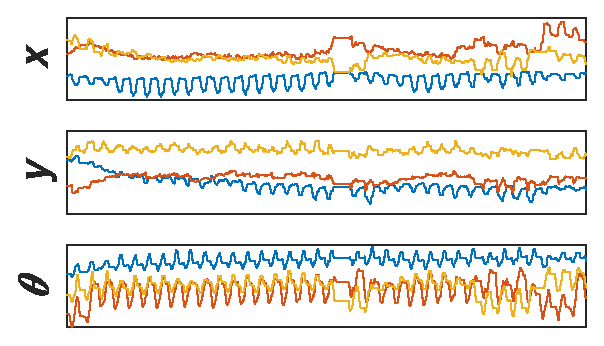
\includegraphics[width=1\textwidth]{crdDat.eps}
		\caption{Time-traces of Smarticle coordinates and angles as tracked from experiments \label{fig:crdDat}}
	\end{subfigure}
	\begin{subfigure}[t]{0.4\textwidth}
		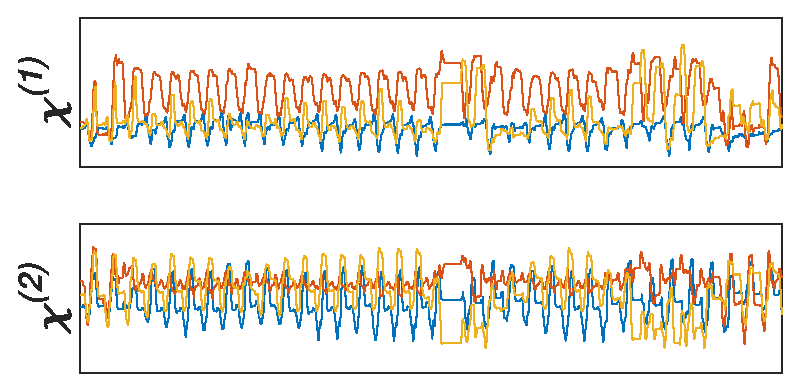
\includegraphics[width=1\textwidth]{relDat.eps}
		\caption{Rotationally invariant observables: c.o.m. coordinate as seen in the reference frame of each smarticle \label{fig:relDat}}
	\end{subfigure}
	\begin{subfigure}[t]{0.4\textwidth}
		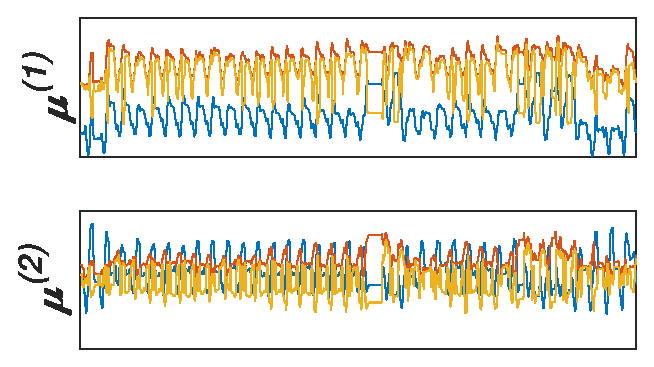
\includegraphics[width=1\textwidth]{piDat.eps}
		\caption{Permutation invariant observables: first 3 moments of the distributions in \ref{fig:relDat} \label{fig:piDat}}
	\end{subfigure}
	\begin{subfigure}[t]{0.5\textwidth}
		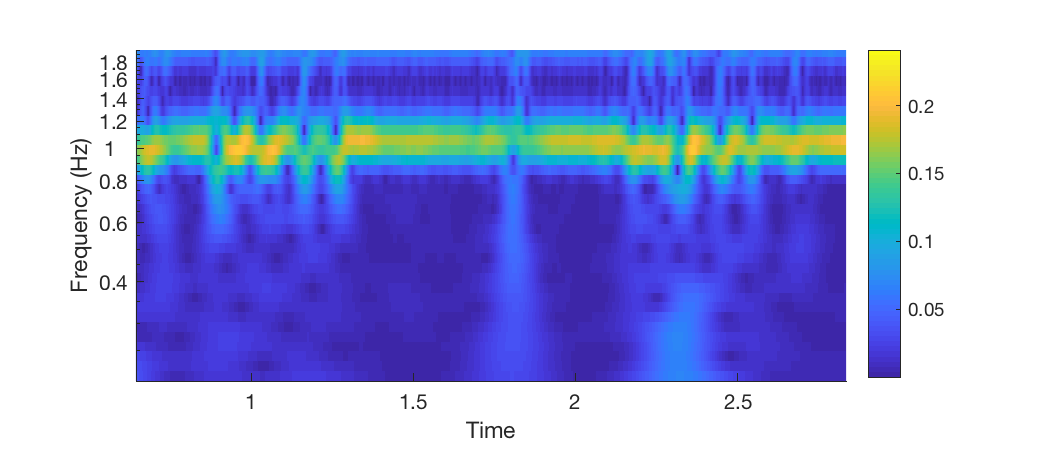
\includegraphics[width=1\textwidth]{wavelet.eps}
		\caption{Wavelet transform of one of the curves in \ref{fig:piDat}. We choose the values along the bright line for our feature vector. \label{fig:waveletDat}}
	\end{subfigure}
	
	\caption{Data processing steps} \label{fig:1}
\end{figure}

\subsection{Modding out symmetries}
We begin by constructing functions of the raw data that are invariant under the symmetries we mentioned, but still sensitive to the information we may care about. The two symmetries are global rotations and permutation. To take care of the first, we find the coordinates of the c.o.m. $ \vec{X}= \frac{1}{3} \sum_i \vec{x}_i $ (note: permutation invariant) in the reference frame of each smarticle: $ \vec{\chi}_i \equiv \mathcal{R}(\theta_i) \cdot (\vec{X} - \vec{x}_i) $, where $ \mathcal{R}(\theta_i) $ is the rotation matrix for $ i $-th smarticle (fig \ref{fig:relDat}). Note that this is not a perfect choice: it is entirely invariant under c.o.m. translations (which is relevant, but we assume it to be small for a confined system), and smarticle orientation matters more the further it is from c.o.m. (so we must assume that their distance to c.o.m. stays relatively constant). We can often get away with such imperfect choices because we have so much overloaded data for the questions. 

Next, the permutation-invariant functions we choose are just the first three moments of the distribution of the three $ \{\chi_i\} $ at any fixed time. In order for these functions to have relatively similar sensitivity to changes in raw data, it helps to ensure that they have the same units -- by raising them to the appropriate fractional powers. I.e., $ \mu_1 = \frac{1}{3} \sum_i \chi_i $, $ \mu_2 = \sqrt{\frac{1}{3} \sum_i (\chi_i-\mu_1)^2} $, $ \mu_3 = \sqrt[3]{\frac{1}{3} \sum_i (\chi_i-\mu_1)^3} $ (fig. \ref{fig:piDat}). Note also that up to 3, these are the same as the cumulants -- which may be a better alternative for more smarticles.

\subsection{Capturing dynamics}
Now we can proceed to dealing with the fact that behaviors we are looking for are dynamic states, and thus depend on multiple time-points. We thus want to construct some feature vector that captures the dynamics. The simplest idea of simply stacking $ \mu_i $ at different time-points on top of each other is not obviously wrong, but will give a feature vector that is very sensitive to the noise. Instead, the dynamical features we are looking for are better captured by Fourier modes. Further, since the dynamical phase can change on the time-scale of a few arm oscillations, we don't want to transform the entire time-series, but instead consider a continuous wavelet transform of the data (fig. \ref{fig:wavelet}). This beautifully separates out behaviors on different time-scales, and we can choose our feature vector based on the time-scale(s) we most care about. The simplest choice here is to take the time-scale corresponding to one gait-period -- since most of the activity happens there. Again, this is throwing away lots of data, but since at the end we just care about some low-dimensional behavior space, we are still left with more than enough (including other time-scales had little effect). 

This way our feature vector consists of 6 complex numbers (3 moments for each dimension of the 2D $ \chi $ vector). We do care about relative phase of oscillation in the wavelet transform -- to keep this in the most unbiased way, we simply take the 36 possible differences between the 6 complex numbers, and then take their absolute value. While this makes the feature vector unnecessarily long, this is fine since we only care about the relative distances between these, and duplicate vector components will simply sum up.

\subsection{Dimensional reduction and clustering}
Now that we have our feature vector, we can dimensionally reduce or cluster the data. The former is, in a sense, a ``smoother,'' less dramatic operation, and thus turns out to produce more accurate results. We can understand this by realizing that in either case, the goal is to preserve pair-wise distances as best as possible, and this is much easier to accomplish if you allow points to be placed anywhere in the $ \mathbb{R}^2 $ plane, rather than in one of 5 discrete states. Curiously, clustering even works better when performed on dimensionally reduced, rather than original data. The other advantage of dimensionally reducing first is that this gives us more information about how the data is distributed, without imposing the assumption that it is well-clustered. 

\begin{figure}
	\begin{subfigure} [t]{0.45\textwidth}
		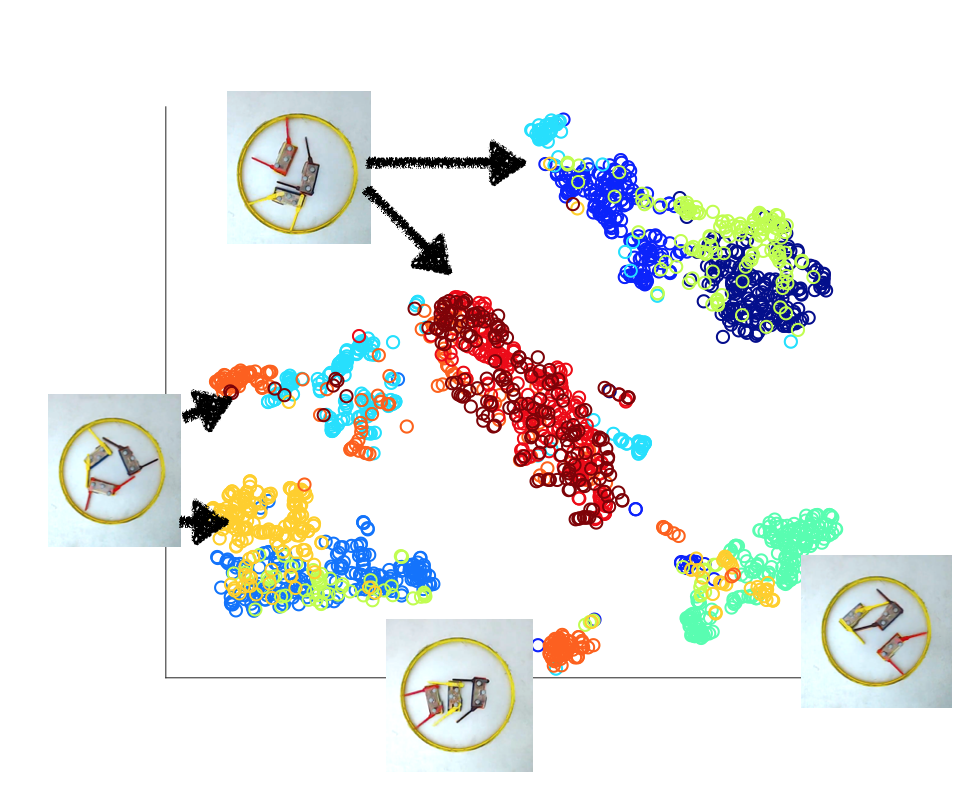
\includegraphics[width=\textwidth]{dimRedExp.png}
		\caption{Experiment \label{fig:dimRedExp}}
	\end{subfigure}
	\begin{subfigure} [t]{0.45\textwidth}
		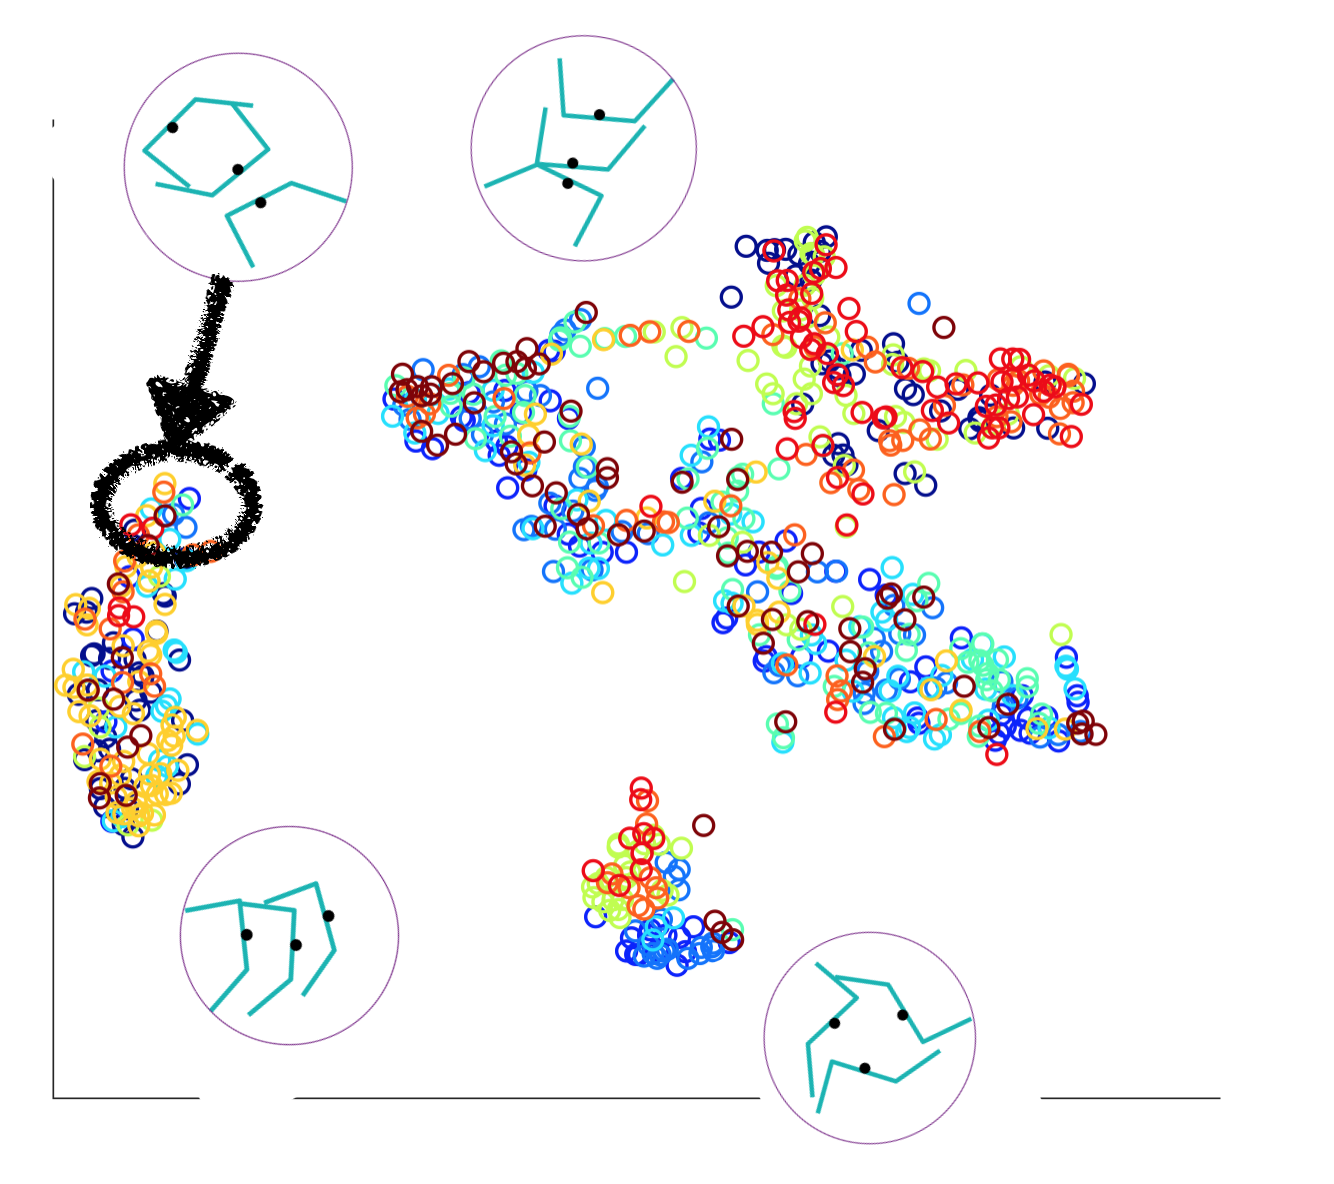
\includegraphics[width=\textwidth]{dimRedSim.png}
		\caption{Simulation \label{fig:dimRedSim}}
	\end{subfigure}
	\caption{Dimensionally reduced data. Insets show what sort of behavior each cluster corresponds to. Note that the cluster positions in the two plots are unrelated as the 2D embedding was done separately on two data sets. Color indicates different trials of the same experiment -- confirming that the behaviors are reproducible.}
\end{figure}

We use Matlab's built-in t-Distributed Stochastic Neighbor Embedding (tSNE) algorithm, which basically tries to embed the data in a 2D space preserving all the pair-wise distances as much as possible (fig. \ref{fig:dimRedExp}). It has the effect of largely preserving, or even highlighting, clusters in the original data, but also allows visualizing transitions between them and other hierarchical structure in the data. Note that the two pairs of clusters corresponding to the same pictures are chiral complements (the other two clusters correspond to non-chiral states). In section \ref{sec:dynPhaseTrans} below we will cluster this data and study the slow transition statistics between different dynamical phases.

\section{Defining Rattling} \label{app:defRatt}

While the intuition that things end up in ``colder'' regions seems simple, it is not immediately clear how we should define a scalar quantity that would be quantitatively predictive of the steady-state probability density for a range of values -- not just as a binary ``high-low.'' Consider the general diffusion process:
\begin{align} \label{eq:MAID}
 \dot{x}_i = D_{ij}(x)\cdot \xi_j \quad \mbox{[It\^o]}
\end{align} 
where $ \xi_i(t) $ - univariate Gaussian white noise: $ \<\xi_i\>=0 $ and $ \<\xi_i(t),\xi_j(s)\>=\delta_{ij}\,\delta(t-s) $, indices $ \{i,j,k,n,m\} $ run over the $ d $ dimensions of the configuration space, and temperature tensor is defined as $ T(x) \equiv \frac{1}{2} D\, D^T $. By analogy wit these dynamics, we could define effective temperature more generally as $ T_{ij}(x) = \frac{1}{2}\int ds \; \<\dot{x}_i(t),\dot{x}_j(s) \> $. However, it isn't a-priori clear what the range of integration should be, if any, especially if correlations don't really drop to zero, whether we should be taking only the connected part of this correlator, and what's the right way to construct a scalar from this so we can talk about $ p_{s.s.} $. Additionally, we want to somehow filter out, at least partly, the periodic or cyclical part of the motion, which does not produce any probability drop. 

\subsection{As inference problem} \label{app:inferT}

One perspective we can take on addressing these issues is by solving the following concrete problem. Let's assume that the underlying motion is indeed Brownian, governed by eq.\ref{eq:MAID}, and we want to infer the inhomogeneous temperature tensor $ T(x) \equiv \frac{1}{2} D\, D^T $ from observations of trajectories. This amounts to a Bayesian inference problem: $ P\[T(x)\,|\,x(t)\]= P\[x(t)\,|\,T(x)\]\, P\[T(x)\]/Z $ ($ Z = P[x(t)] $ -- normalization). For our prior $ P\[T(x)\] $, we assume that temperature landscape varies smoothly over $ x $ -- otherwise we can never hope to estimate it from a finite observation of trajectory. Explicitly, this can be implemented via: $ P\[T(x)\] \propto \exp{-\epsilon \int d^d x\; \partial_k T_{ij} \partial_k T_{ij}}$. Additionally, from the distribution for Gaussian white noise, we get $ P\[x(t)\,|\,T(x)\] = \prod_t \[ \sqrt{\frac{1}{\det(4\pi T)}}\,\exp{-\frac{1}{4} T^{-1}_{ij}\dot{x}_i \dot{x}_j} \]$ this way:
\begin{widetext}
\begin{align*}
 P\[T(x)\,|\,x(t)\] = \frac{1}{Z[x(t)]} \; \exp{-\int dt \[\frac{1}{2}\, \tr \log T(x(t)) + \frac{1}{4}\, T^{-1}_{ij}(x(t))\;\dot{x}_i(t)\,  \dot{x}_j(t)\]-\epsilon \int d^d x\; \partial_k T_{ij}\partial_k T_{ij}}
\end{align*}
\end{widetext}
Note that, interestingly, we have an integral over time and another integral over configuration space in the exponent. We then want to choose some estimator for $ T(x) $. The easiest to evaluate here is the maximum-likelihood, which we can get by setting the variation $ \fd{\quad}{T(x)} $ of the exponent to 0, which gives:
\begin{align*}
4\epsilon\, \left. T_{in}T_{jm} \partial_k^2 T_{mn}\right|_X = T_{ij}(X) - \frac{1}{2}\<\dot{x}_i(t)\,  \dot{x}_j(t)\>_{t\; |\;x(t)=X}
\end{align*}
where the average is over all the times when trajectory $ x(t) $ passes through $ X $. So if we had a uniform prior $ \epsilon\rightarrow 0 $, then we get that $ T_{ij}(X) $ is simply the equal-time second-moment of velocity trajectories have at that point. For $ \epsilon>0 $, any deviations from this rule become sources for a diffusions equation, smoothing out the landscape -- and thus for small $ \epsilon $, we simply get that the average $ \<\cdot\> $ above is not only at $ X $, but over its neighborhood, weighted by a Gaussian kernel: 
\begin{align} \label{eq:Tij}
T_{ij}(X) = \frac{1}{2}\<\dot{x}_i(t)\,  \dot{x}_j(t)\>_{t\; |\;(x(t)-X)^2 \,<\, \epsilon}.
\end{align} 

Now, we can use this result to take our trajectories $ x_i(t) $, which come from some non-diffusive dynamical system, and infer the temperature landscape that might have created such trajectories. This will always produce some result, regardless of how poor of a model diffusive behavior is for our dynamics. But if we do want to use the diffusive approximation, then this shows that we need only consider the equal-time correlator, rather than the integrated one. 

\subsection{Max-entropy modelling} \label{app:max-ent}

To motivate this diffusive approximation better, we can view it as maximum entropy modelling (or more precisely, ``maximum caliber,'' as in \cite{dill18max_caliber}). We ask, if we knew nothing about our dynamics besides the amplitude of fluctuations (2-point correlators) throughout the configuration space, what would be our most unbiased guess at what the dynamics really are? We can frame this question precisely by finding the maximum-entropy probability distribution over the space of possible trajectories $ \{x(t)\} $, under the constraint that two-point correlators match the data. As with all maximum-entropy modelling the result depends crucially on what we choose to constrain -- even with two-point functions, we have the freedom to choose between equal-time correlator, integrated correlator, different choices of spatial averaging, etc. Motivated by the above inference result (eq.\ref{eq:Tij}), we will first try to constrain the equal-time correlator at every point in configuration space. Thus the entropy functional we want to maximize w.r.t. $ P[x(t)] $ is:
\begin{widetext}
\begin{align*}
\mathcal{S} = P[x] \;\log\(P[x]\) + \lambda_0 \(1- \int \mathcal{D} x \;P[x]\) + 
\int dX \; \lambda_{ij}(X) \(\frac{1}{2}\< \dot{x}_i\,\dot{x}_j\> _X - T_{ij}(X)\)
\end{align*}
\end{widetext}
where $ \< \dot{x}_i\, \dot{x}_j\> _X \equiv \int \mathcal{D}x \; P[x] \,\int dt \; \dot{x}_i(t) \dot{x}_j(t) \,\delta(x(t) - X) $, and $ T_{ij}(X) $ is the corresponding quantity measured from the data. $ \lambda_0 $ and $ \lambda_{ij}(X) $ are Lagrange multipliers for the normalization and fluctuation constraints. As in the inference section above, we have an interesting mix of integrals over configuration space and over trajectory duration. Setting the variation $ \fd{\quad}{P[x]} $ to 0, we get:
\begin{widetext}
	\begin{align}
	&1+ \log(P[x])+\lambda_0 + \int dX \; \lambda_{ij}(X) \int dt \; \dot{x}_i(t) \dot{x}_j(t) \,\delta(x(t) - X) =0\\
	&\Rightarrow \qquad P[x]=\exp{-1-\lambda_{0}-\int dt \; \lambda_{ij}(x(t))\,\dot{x}_i(t) \dot{x}_j(t) } \label{eq:maxEnt}
	\end{align} 
\end{widetext}
We must then set the Lagrange multipliers such that our constraints are satisfied. This means that $ \lambda_0 $ is chosen to give proper normalization, and $ \< \dot{x}_i\, \dot{x}_j\>_X = \frac{1}{2}\lambda^{-1}_{ij}(X) = 2 \,T_{ij}(X)$, giving us $ P[x]=\frac{1}{Z}\; \exp{-\frac{1}{4}\int dt \; T^{-1}_{ij}(x(t)) \,\dot{x}_i(t) \dot{x}_j(t)}  $. But this is precisely the probability distribution for the diffusive dynamics we had in eq.\ref{eq:MAID}! 

We can thus view our diffusive dynamics assumption as the natural unbiased approximation reproducing the 2-point correlators of the actual dynamics. It is curious to note here that this derivation is surprisingly fragile to the choice of constraint. If instead of the equal-time correlator (eq.\ref{eq:Tij}) we chose to constrain anything else, such as integrated correlator, we would have no way to easily express $ \lambda_{ij}(X) $ in terms of $ T_{ij}(X) $ -- and in particular, the dependence would be non-local! This is because the distribution in eq.\ref{eq:maxEnt} is non-Gaussian, and so the two-point correlator is not in general simple. 

\subsection{Filtering out periodic motion}
Clearly, the diffusive approximation badly fails if you have motion around a limit-cycle. In this case, you exit a particular region of configuration space, only to come back there every time, and so without suppressing the steady-state probability of that region. Statistically, this break-down between exit rates and $ p_{s.s.} $ happens because entrance rates become strongly correlated with exit rates (see sec.\ref{app:randMarkov}). Either way, we need some way to filter out periodic motion from our estimates of effective temperature. To proceed, we can express our velocity, whose correlators we've been studying, in frequency space as $ \dot{x}_i = \Im\[\int d\omega \; \omega\, x_i(\omega)\] $. The evolution of this spectrum over time is basically what's plotted in fig.\ref{fig:reg}b. We can then try to filter it in different ways to remove any regular part of the motion. 

For systems with periodic driving, we can simply suppress all signal at the driving frequency -- this does not guarantee that other emergent periodicity cannot happen, but it will remove the dominant source of regularities. In general, there is no objective way to tease apart regular from chaotic behaviors -- since to some extent it depends subjectively on the time-scale of observation of your system.  This is famously illustrated by the Fermi–Pasta–Ulam paradox, where dynamics that seemed chaotic at first, turned out to be exactly periodic on a longer time-scale. This is the key point where we rely on our assumption of ``complexity:'' we assume that typically, for real many-body interacting systems, the probability of a trajectory returning to an earlier configuration is indistinguishable from chance, after a sufficiently long delay time. Note that this is a strictly weaker assumption than saying that complex systems lose memory of where they were over time -- in fact, the entire point of this paper is to discuss what sort of long-term memory effects we can expect in such systems. 

This thinking does motivate another way to estimate effective temperature from velocity spectrum: since we believe that most periodicity or organization in such systems should happen on faster time-scale, we can simply use a low-pass filter. E.g., in the wavelet transform of fig.\ref{fig:reg}b, we see the noise-component of the dynamics showing up as the broad-band in the lower-frequency range. Similarly, we can simply define the noise component as the broad-band part of the power-spectrum, after removing any sharply-peaked (narrow-band) features. This is also motivated by the intuition that white-noise is distinguished by having power at all frequencies. 

This way, while at this point, we cannot make a precise argument for how to reliably separate out the truly chaotic part of the dynamics, there are a number of reasonable guesses we can make. Most definitively, we can say that at the end of the day, our chosen definition of effective temperature does seem to be predictive of the steady-state in our experiments. Moreover, this correlation remains largely unchanged for the different choices listed in this section. 

\subsection{Constructing a scalar} \label{app:rattScalar}

With the above methods, we motivated how to measure effective temperature tensor $ T_{ij}(x) $ from the trajectory data. To predict the steady-state distribution, however, we must first convert this to a scalar $ \mathcal{R}(x) $, which we call Rattling, with the hypothesis that $ p_{s.s.}(x)\sim 1/\mathcal{R}(x) $. Note that no result like this can hold exactly in general, as the diffusion process in eq.\ref{eq:MAID} does not generally admit a closed-form analytical solution for the steady-state. This can be understood by recognizing that this stochastic process is generally not detailed-balanced, and so $ p_{s.s.}(x) $ can depend non-locally on values of $ D_{ij}(y) $ anywhere.

Thus, all we can hope to get is an approximation of $ p_{s.s} $, and we can thus be motivated in the choice of an approximation by studying solvable limiting behaviors. The two leading candidates for a scalar that could work here are the trace of $ T_{ij} $ and its determinant. As we have not yet been able to conclusively decide which of these two is more generally appropriate, following we present the arguments in favor of each choice.

The first argument to use the trace comes from the fact that for the isotropic limit of diffusion in eq.\ref{eq:MAID}: 
\begin{align} \label{eq:MIID}
\dot{x}_i = \sqrt{2\,T(x)}\cdot \xi_i
\end{align}
 (i.e., if the temperature tensor $ T_{ij}(x) = \delta_{ij}\,T(x) $), we get the Fokker-Planck equation $ \dot{p} = \partial_i^2(T(x)\, p) $, whose steady-state is $ p_{s.s.}\propto 1/T(x) \propto 1/\tr[T_{ij}(x)]$. Note that determinant here would $ = T^d $, with $ d $ -- dimensionality of configuration space, and so would not work here. The numerical tests in sec.\ref{app:randDiff} also support that $ p_{s.s.}\propto 1/\tr[T_{ij}(x)]$.

Another argument in favor of trace comes from noting that if the inference in section \ref{app:inferT} were carried through from the assumption of isotropic temperature, the maximum-likelihood estimator for that scalar temperature would have been $ T(X) = \frac{1}{2}\, \sum_i \<\dot{x}_i(t)\,  \dot{x}_i(t)\>_{t\; |\;(x(t)-X)^2 \,<\, \epsilon} = \tr\[T_{ij}(X)\] $. Similarly, in section \ref{app:max-ent}, if instead of constraining the tensor $ \< \dot{x}_i\, \dot{x}_j\> _X $, we chose to constrain its trace, we would have landed again on eq.\ref{eq:MIID}, but if we instead chose to constrain its determinant, we could not arrive at any local closed-form result due to the additional non-linearity of determinant.

The determinant, on the other hand, is nice in that it is consistent with composite systems. I.e., if we have two independent subsystems with $ p^{(1)}_{s.s.}(x) \propto 1/\det\[T^{(1)}\]$ and $ p^{(2)}_{s.s.}(y) \propto 1/\det\[T^{(2)}\]$, then the total $ p_{s.s.}(x,y)=p^{(1)}_{s.s.}(x) \, p^{(2)}_{s.s.}(y) \propto 1/\det\[T^{(1)}\,T^{(2)}\]$. In particular, if the temperature tensor takes the form $ T_{ij}(\vec{x})=\delta_{ij}\,T_i(x_i) $, where its $ i $-th component is independent of all $ \{x_j\}_{j\ne i} $, then the Fokker-Planck equation $ \dot{p} = \sum_i \partial_i^2 \(T_i(x_i)\, p\)$ has the steady-state $ p_{s.s.} \propto \prod_i 1/T_i(x) = 1/\det\[T_{ij}(x)\] $. We thus see that for different $ x $-dependencies of the temperature tensor, $ 1/p_{s.s.}(x) $ can be proportional to either the trace or the determinant -- we explore this cross-over directly in section \ref{app:randDiff} below.

Another evidence in favor of the determinant is its behavior under coordinate-changes. This is of crucial importance, since the estimation of $ T_{ij} $ in eq. \ref{eq:Tij} is entirely dependent on how we choose to parametrize our data. In particular, looking at all the coordinate transformations described in appendix \ref{app:dataAnal}, we clearly see that the data parametrization we use to produce the plots in this paper is anything but simple or linear in any way -- and so the fact that the correlations still hold indicates the relationship must be reparametrization invariant. Concretely, if we change variables $ x_i \rightarrow y_i(\vec{x}) $, then the probability density picks up the Jacobian of the transformation $J(y) \equiv \det\[\partial^i y_j\] $ (where partial derivative is w.r.t. $ x $-coordinates), such that $ p_{s.s.}(x) \rightarrow \tilde{p}_{s.s.}(y)=p_{s.s.}(x(y))/J(y)$. Temperature tensor, on the other hand, transforms $ T_{ij}(x) \rightarrow \tilde{T}_{ij}(y)=T_{kl}(x(y)) \partial^k y_i\partial^ly_j$, and so $ \det\[\tilde{T}_{ij}\] = J^2 \det\[T_{ij}\] $. This way, the expression $ p_{s.s.}(x) \propto 1/\sqrt{\det\[T_{ij}(x)\]} $ is reparametrization-invariant. But what about this square root?

We must also remember that by It\^o's lemma, a change of coordinates also introduces drift terms, such that the correct $ y $-dynamics for eq.\ref{eq:MAID} are $ \dot{y}_i = T_{jk}\,\partial^j\partial^k y_i + \partial^k y_i `D_{k}^{j}`\cdot\xi_j $. Thus, for 1D, or for 1D systems composed together as above, this drift ensures the correct transformation of the expression $ p_{s.s.}(x) \propto 1/T(x) $. In high dimensions, we could argue that unless the coordinate change is fine-tuned to the profile of $ T_{ij}(x) $, these drift terms may be small -- but also they are correlated with magnitude of $ T_{ij} $, and so may have a substantial effect on $ p_{s.s.} - T$ correlation.

In all, it seems that the correct way to construct a scalar for rattling (such that $ p_{s.s.}\sim 1/\mathcal{R} $) may depend on the statistics of disorder in our dynamical system. Empirically, $ \mathcal{R} = \det\[T_{ij}\] $ seemed to be the most robust choice for the smarticle system above -- though we see some cases where the power $ p_{s.s.} \sim 1/\mathcal{R}^p $ deviates from 1, e.g., fig.\ref{fig:otherRun}a. In appendix \ref{app:randDynam} we explore other examples of dynamical systems where different choices for $ \mathcal{R} $ may be more reliable.

\section{Random dynamical systems} \label{app:randDynam}

In this section, we attempt to make more precise statements about ``typical'' dynamical systems and their steady-states by randomly constructing and analysing various types of such systems. With some of these we can make analytical progress, with others we must mostly resort to numerics. The general theme we are focusing on here is that while the exact steady-state at a point $ p_{s.s.}(x) $ will depend non-locally on system properties throughout configuration space, we can often construct a local observable (i.e., rattling $ \mathcal{R}(x) $), which is approximately predictive of the steady-state. 

\subsection{Random Markov process} \label{app:randMarkov}

While we have up to this point only talked about dynamical systems with continuous state-space, the easiest example of random dynamics we can solve is a Markov process on $ N $ discrete states. Consider the master equation $ \dot{p}_i= \sum_j R_{ji}\, p_j - \sum_j R_{ij}\, p_i $, with $ i\in\{1,...,N\} $ labeling states. In general the steady-state distribution $ p_{s.s.}(i) $ is the null eigenvector of the transition-graph Laplacian matrix $ L_{ij}= -R_{ji} + \sum_j R_{ij} $, and thus will depend in a complicated way on all the $ N^2 $ transition rates. 

Now, as we want to understand large disordered dynamical systems, we let the transition rates $ R_{ij} $ be independent identically distributed random variables, with some mean $ \bar{R} $ and standard deviation $ \sigma $, and let $ N \rightarrow \infty$. We now want to try finding the steady-state as an asymptotic series in powers of $ \frac{1}{N} $: $ p_{s.s.}(i) = p^{(0)}_i + p^{(1)}_i +... $. First, by the central limit theorem, we can write the mean entrance and exit rates for state $ i $ as:
\begin{align*}
\frac{1}{N} \sum_j R_{ji} = \bar{R} + \frac{\sigma\, \xi_i}{\sqrt{N}}\\
 \frac{1}{N} \sum_j R_{ij} = \bar{R} + \frac{\sigma\, \zeta_i}{\sqrt{N}}
\end{align*}
respectively, where $ \xi_i $ and $ \zeta_i $ are univariate Gaussian random variables specifying the deviation of $ i $-th entrance and exit rate from the mean. We immediately see that at leading order, constant $ p^{(0)}_i =\frac{1}{N} $ is a self-consistent choice:
\begin{align*}
\dot{p} = \sum_j R_{ji}\, \frac{1}{N} - \sum_j R_{ij}\, \frac{1}{N} =  \bar{R} + \frac{\sigma\, \xi_i}{\sqrt{N}} - \bar{R} - \frac{\sigma\, \zeta_i}{\sqrt{N}}
\end{align*}
which vanishes for large $ N $. The first correction to the steady-state must further reduce $ \dot{p} $:
\begin{align*}
\frac{\sigma\, (\xi_i-\zeta_i)}{\sqrt{N}} +\sum_j R_{ji}\, p^{(1)}_j - \sum_j R_{ij}\, p^{(1)}_i \sim o\(\frac{1}{\sqrt{N}}\)
\end{align*}
(using the little-o notation). We can check that letting $ p^{(1)}_i =  \frac{\sigma\, (\xi_i-\zeta_i)}{\bar{R}\, N^{3/2}}$ accomplishes this:
\begin{align*}
\sum_j R_{ji}\, p^{(1)}_j - \sigma\, \zeta_i\; p^{(1)}_i\,\sqrt{N} \sim o\(\frac{1}{\sqrt{N}}\)
\end{align*}
where the second term is explicitly of $ \bigO{\frac{1}{N}} $, and the first term averages out to be of that order if $ R_{ji} $ is uncorrelated with $ p^{(1)}_j $. 

This last assumption is the crucial step of the derivation, and plays a similar role to that of the molecular chaos assumption in equilibrium thermodynamics. In particular, it breaks time-reversal symmetry by distinguishing between exit and entrance currents for a given state $ i $: the former are all correlated as they are all $ \propto p^{(1)}_i $, while the latter average out as they are proportional to the independent random variables $ p^{(1)}_j $. In reality, this assumption does not exactly hold, as $ p^{(1)}_j $ depends on $ j $th exit rate $ \zeta_j $, which correlates with  $ R_{ji} $ -- but as all the rates are assumed independent, the effect of this correlation is suppressed by an additional factor of $ \frac{1}{N} $. Thus we see that if we introduce correlations in the rates $ R_{ij} $, this assumption will be the first failure mode of the derivation -- but by the same token, as long as it holds, so should our result. 

Putting the pieces together, we thus get the approximate expression for the steady-state 
\begin{align*}
p_{s.s.}(i)= \frac{1}{N} + \frac{\sigma\, (\xi_i-\zeta_i)}{\bar{R}\, N^{3/2}} + \bigO{\frac{1}{N^2}}=\\
\frac{1}{N} + \sum_j (R_{ji} - R_{ij})/(N^2\,\bar{R}) + \bigO{N^{-2}}
\end{align*}
So the steady-state probability at a states depends in an equal measure on both the exit, and the entrance rates of that state. In practice, however, the total entrance rate may be hard to measure, as it would require initializing the system in all possible configurations and seeing how often it enters $ i $. The exit rate, on the other hand, is akin to our measure of rattling -- it is basically a measure of how stable the state $ i $ is and only requires local measurements initialized in that state. While not enough to predict the steady-state exactly, it can already tell us a lot, and will be strongly correlated with it (see fig.\ref{fig:randDynamics})a.

This way, we see that while in general we need all $ N^2 $ rates to predict the steady-state, the randomness in rates and large system size allow us to express it in terms of just $ 2 N $ local measurements of the exit and entrance rates.

\subsection{Diffusion in random medium} \label{app:randDiff}

Here we look more carefully at the generic multi-dimensional diffusion process of eq.\ref{eq:MAID}, reproduced here:
\begin{align} \label{eq:MAID1}
\dot{x}_i = D_{ij}(x)\cdot \xi_j \quad \mbox{[It\^o]}
\end{align} 
with $ T\equiv \frac{1}{2}D\,D^T $. As we cannot find the steady-state analytically, we study this numerically. Again, as we want to study some ``typical'' regime, we choose $ D_{ij}(x) $ landscape randomly, but so that it varies smoothly in $ x $. Explicitly, for each of $ d^2 $ entries of this matrix, we independently generate a random $ d $-dim grid of numbers $ \in(-1,1) $ (e.g., for $ d=4 $, this may be $ 5\times5\times5\times5 $), and then use cubic interpolation to fill in the values in-between, thus making a smooth landscape (e.g., making a $ 15\times15\times15\times15 $ grid). To then find the steady-state distribution, we explicitly construct the discretized Fokker-Planck operator $ \partial_i\partial_j\(T_{ij}(x) \,\cdot\,\) $ as a matrix, implementing periodic boundary conditions, and find its null eigenvector. Note that if we now view this matrix as the Laplacian matrix of a Markov jump process, as in section \ref{app:randMarkov} above, then the exit rates found on the diagonal, will be simply $ \tr\[T_{ij}\] $ (though this could be slightly different depending on the choice of discretization). Plotting the computed exact steady-state vs. trace or determinant of $ T_{ij} $ (fig. \ref{fig:randDiff}), we see that for this setup, trace correlates much better, and unlike determinant, scales linearly with $ p_{s.s.}^{-1} $. The correlation becomes more pronounced if, after constructing the diffusion tensor $ D_{ij}(x) $ as described above, we raise it to the 4th power to amplify its variation over $ x $ (fig.\ref{fig:randDiff4D_p4}).

\begin{figure} 
	\begin{subfigure}[t]{0.5\textwidth}
		\caption{\label{fig:randDiff4D}}
		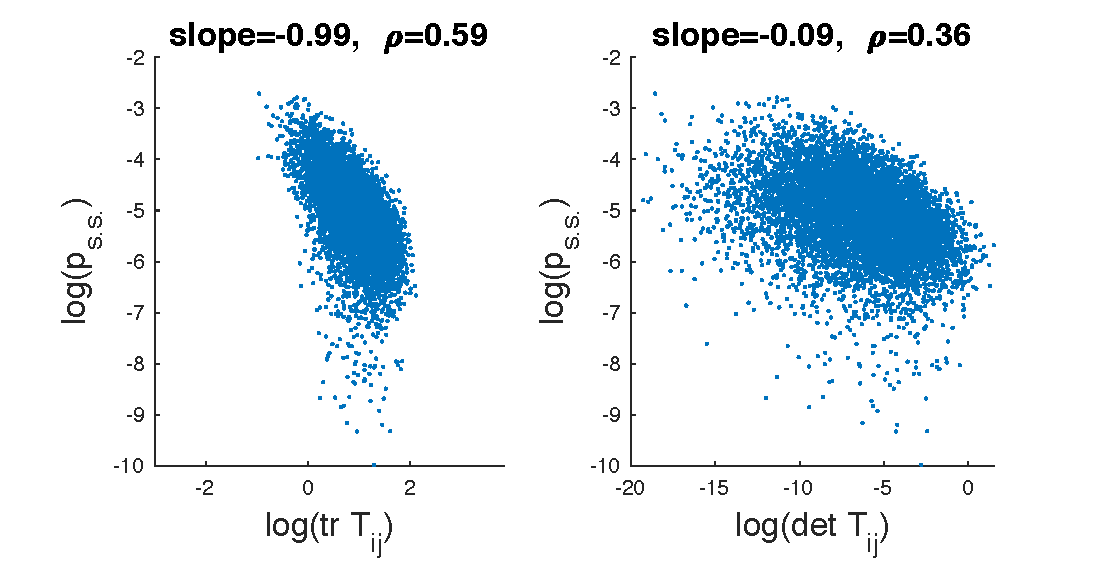
\includegraphics[width=1\textwidth]{randDiff4D.pdf}
	\end{subfigure}
	\begin{subfigure}[t]{0.5\textwidth}
		\caption{\label{fig:randDiff4D_p4}}
		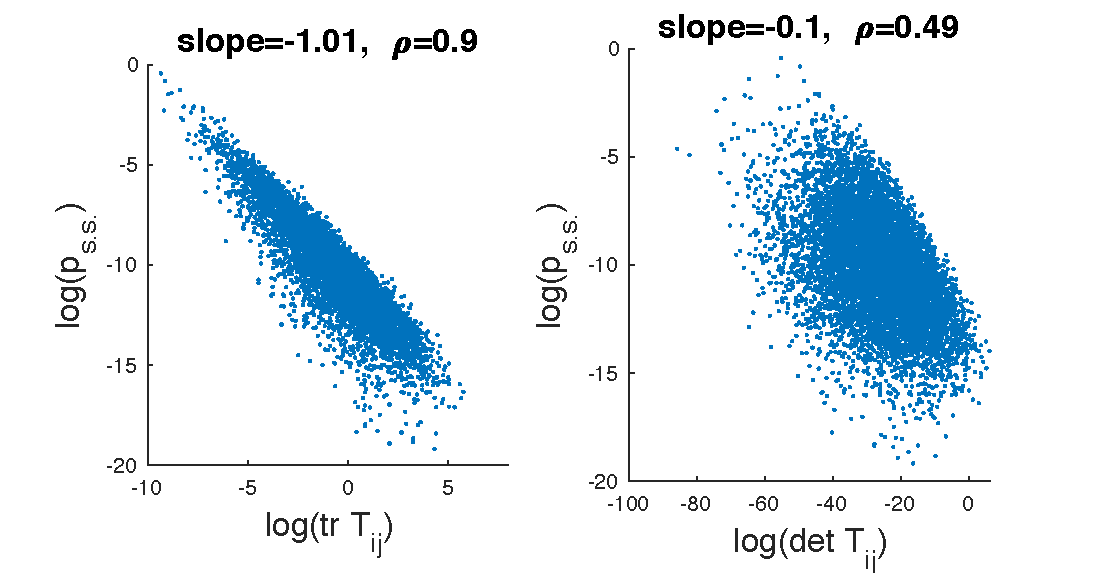
\includegraphics[width=1\textwidth]{randDiff4D_p4.pdf}
	\end{subfigure}
	\caption{Numerical results for 4D diffusion process in eq.\ref{eq:MAID1} with randomly varying diffusion tensor $ D_{ij}(x) $. (b) shows results when $ D(x) \rightarrow D^4(x) $ to allow larger amplitude variation. Linear regression slopes and correlation coefficients are listed above.} \label{fig:randDiff}
\end{figure}

We can run a couple other tests with this setup. First, we claim that this correlation crucially relies on the disorder and ``typicality'' of our chosen dynamics. Thus, we should be able to break it by introducing some fine-tuning or correlations into the diffusion landscape. In particular, if we have strong diffusion along a closed ring, then while $ \tr\[T_{ij}\] $ will be large there, it will not contribute to any suppression of $ p_{s.s.} $ as trajectories don't leave that ring any more frequently. We implement this scenario in 2D (for better visualization -- works same way in higher dimensions), as shown in fig. \ref{fig:randDiff2D_br}, second panel. We also see in the third panel that if the direction of enhanced diffusion is not aligned along the ring, then the correlation is restored -- illustrating that breaking it really requires strong fine-tuning.

\begin{figure} 
	\begin{subfigure}[t]{0.5\textwidth}
		\caption{\label{fig:randDiff2D_br}}
		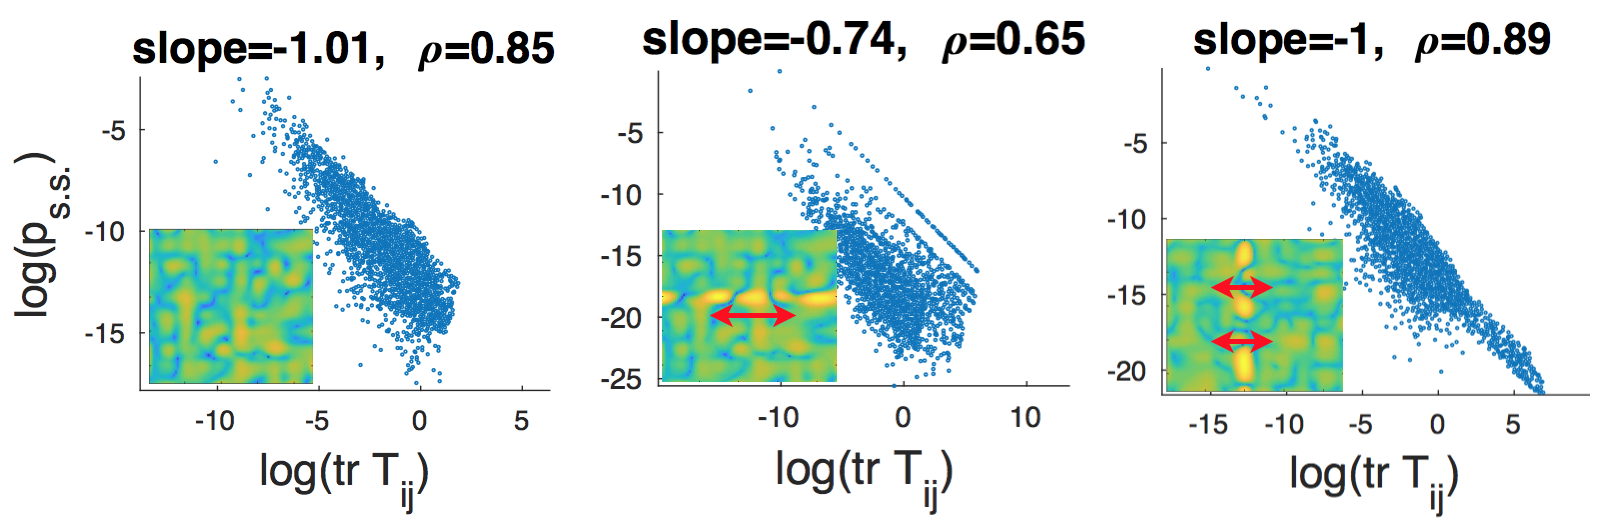
\includegraphics[width=1\textwidth]{randDiff2D_break.png}
	\end{subfigure}
\begin{subfigure}[t]{0.5\textwidth}
	\caption{\label{fig:trVdet_crossover}}
	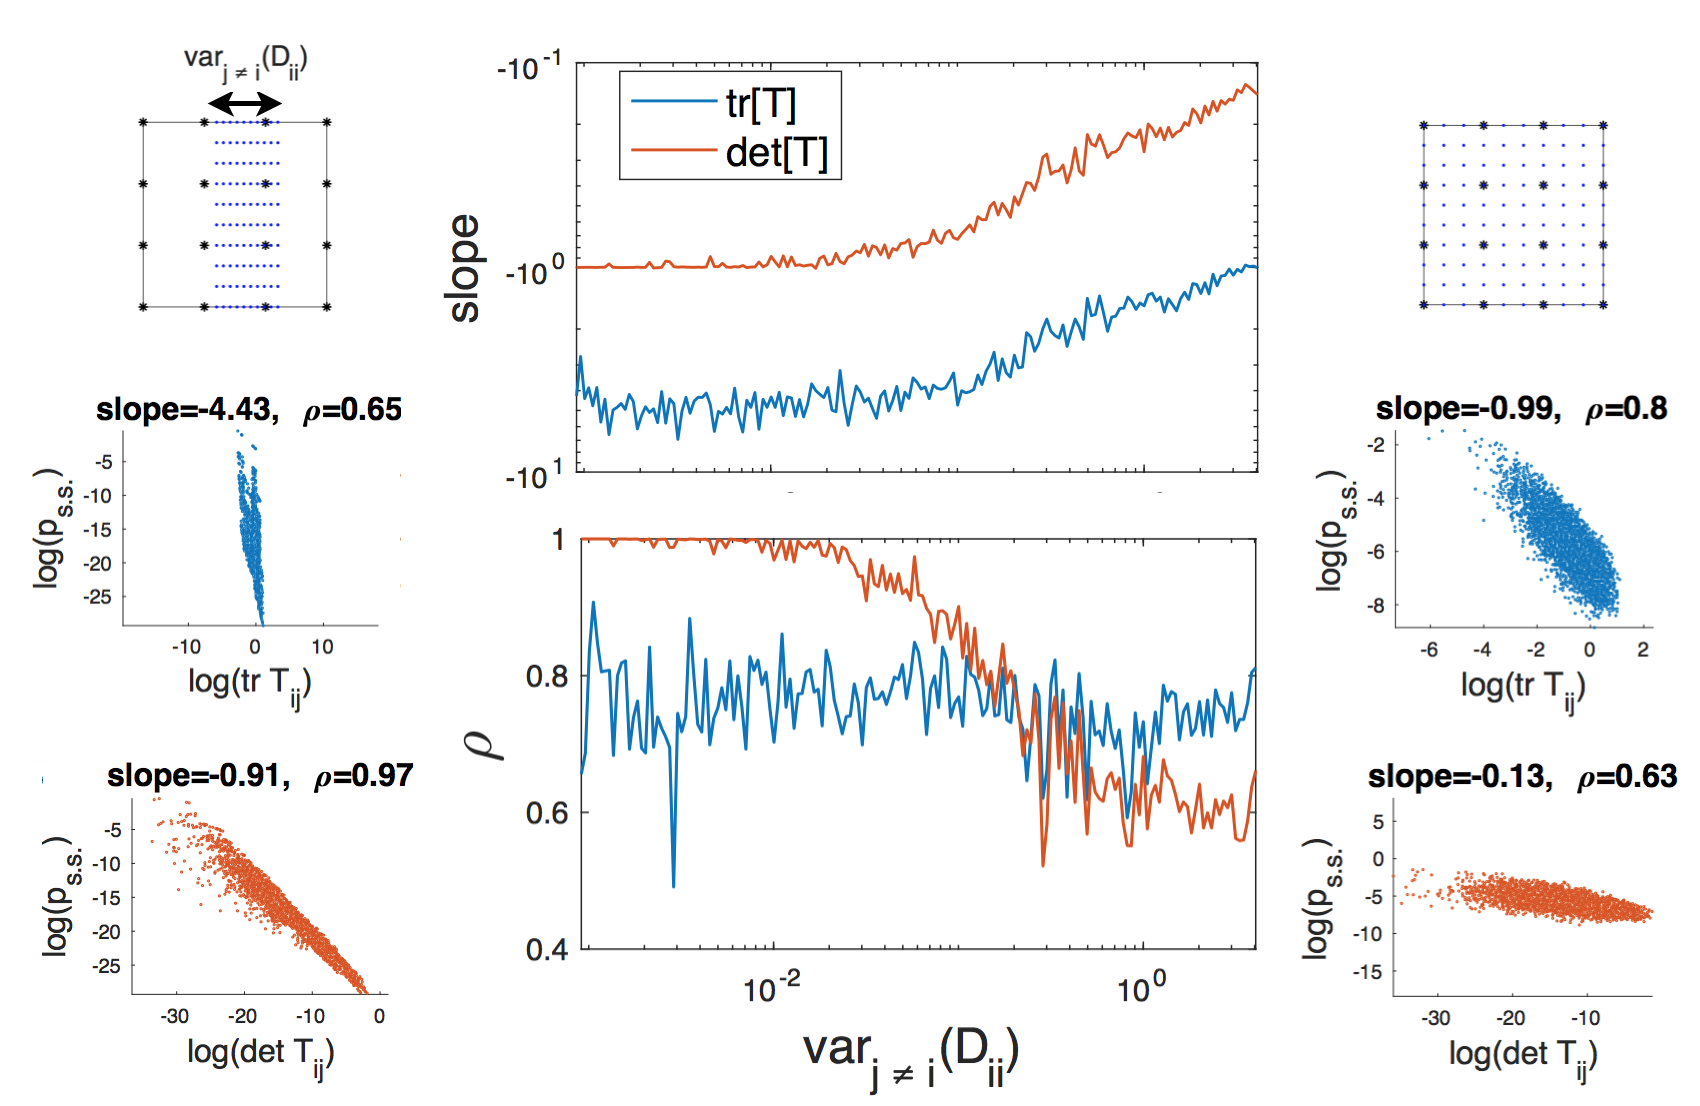
\includegraphics[width=1\textwidth]{trVdet_crossover.png}
\end{subfigure}
	
	\caption{(a) Breaking the correlation by enhancing diffusion along a closed ring (in 2D). Insets show the $ \log\tr\[T_{ij}(x)\] $ landscape (boundaries are periodic, so the bright bands are actually closed). Three panels show respectively the setups with diffusion unperturbed random, enhanced along the ring, and orthogonal to the ring -- only the second case breaks the correlation. (b) Crossover from determinant to trace being predictive of $ p_{s.s.} $ as variation of $ D_{ii} $ along $ x_{j\neq i} $ dimensions is scaled up, showing the change of regression slope and correlation coefficient. Point grids illustrate how $ D_{yy} $ landscape is generated: random numbers are generated at black stars, and then cubic interpolation is taken at the blue query points, which form the landscape.} \label{fig:randDiff_more}
\end{figure}

Another correlation that we can introduce to the diffusion landscape to change our result is to make it a product of $ d $ 1D diffusion processes -- in which limit we expect $ p_{s.s.}\propto \det\[T_{ij}\] $, as discussed in section \ref{app:rattScalar}. Since thus far we've shown the trace is the one that is inversely linear with $ p_{s.s.} $, this would mean that we should see a crossover between the two regimes. To achieve that limit, let's first restrict $ D_{ij} $ to be diagonal, and then ensure that $ D_{ii} $ does not vary along all $ x_{j\neq i} $ dimensions. We can then smoothly tune up this cross variation $ var_{j\neq i}(D_{ii}) $ up to the full dependence $ D_{ii}(\vec{x}) $ to study the cross-over. Numerically, we implement this by first confining all interpolation query points along $ j\neq i $ dimension to a tiny range of the generated random grid (see description above), and then spreading them out to the max range (illustrated by point grids in fig.\ref{fig:trVdet_crossover}). As seen in fig.\ref{fig:trVdet_crossover} for 4D diffusion, we indeed see this crossover in regression slopes of our distributions. As shown by the correlation coefficient plot, on the other hand, despite changing slope, trace remains well-correlated with $ p_{s.s.} $ throughout, while determinant becomes uncorrelated as we approach full $ \vec{x} $-dependence (the regime in fig.\ref{fig:randDiff}).

\subsection{Random force field}

Most continuous dynamical systems can be written as a first-order system
\begin{align} \label{eq:randForce}
\dot{x}_i = F_i(x,t)+\sqrt{2\,T_0}\;\xi_i
\end{align}
If the system is sufficiently complex and high-dimensional, then we can try to gain insight about ``typical'' behaviors by letting the force-field $ F_i(x) $ be random. Turns out we can gain some analytical insights on this problem -- though the full result will still require numerics. 

\subsubsection{Analytics}
We consider a smoothly-varying force-landscape, which we can analytically construct by letting $ F_i(x) $ be Gaussian random field with $ \<F_i(x)\>=0 $ and $ \<F_i(x) F_j(y)\>=G_{ij}(x,y) $ -- some correlation function that decays with $ |x-y| $ (for cleaner notation, we focus on time-independent systems for now). As we are focusing on the effect of forces here, we take temperature to be a uniform scalar. This setup is nice in that if $ G $ decays very quickly in $ |x-y| $, it approximates diffusive behavior, as any trajectory $ x(t) $ experiences nearly independent forces over time. On the other hand, if there are system-spanning correlations in $ F(x) $, then the behavior is more like deterministic chaos, where trajectories separate faster the further apart they already are. We can thus hope to see these limiting behaviors emerge in our results, and try to understand the crossover.

To evaluate a general observable $ \Op[x(t)] $ under disorder averaging, we must compute the partition function
\begin{align*}
Z[h_\Op] = \<\int \D x \; \exp{-\frac{1}{4T}\int dt\, \(\dot{x}_i - F_i(x)\)^2 + h_\Op \Op}\>_{F_i(x)}
\end{align*}
such that $ \<\Op\> = \left.\pd{Z[h_\Op]}{h_\Op} \right|_{h_\Op=0}$. Note that we can take the disorder average directly of $ \<Z\> $, rather that of $ \<\log Z\> $ because by construction our probabilities are already normalized, as $ Z[h_\Op=0]= $ const. independent of $ F_i(x) $. In a sense, time takes on the role of a replica-index, and just as we get replica-coupling, we will see that here we get global time-coupling.

Evaluating the disorder average we thus get:
\begin{widetext}
	\begin{align*}
Z[h_\Op] = \int \D x \; \mbox{exp}\Bigg[ &-\frac{1}{4T}\int dt\, \(\dot{x}_i^2 + G_{ii}(x,x)\) + 
	\frac{1}{(4T)^2}\iint dt\, ds \(\frac{1}{2} G_{ij}^2\(x(t),x(s)\) + 2\, \dot{x}_i(t) \dot{x}_j(s) G_{ij}\(x(t),x(s)\)\) - \\
	&-\frac{1}{(4T)^3}\iiint dt\, ds\, du \;\frac{2}{3} \dot{x}_i(t) \dot{x}_j(s) G_{ik}\(x(t),x(u)\) G_{jk}\(x(s),x(u)\) + h_\Op \Op \Bigg]
\end{align*}
\end{widetext}
While this looks bad, it turns out we can build substantial intuition for the various terms if we think of it as a partition function for a polymer. From this perspective, the first integral just gives the energy of a Gaussian coil in an energy landscape given by $ \tr\[G(x)\] $ -- i.e., the polymer avoids regions with large amplitude $ F_i $, as the trajectory tends to leave these. The double integral then gives polymer self-interaction energy: the first term is an attractive force with range set by $ F(x) $ correlation length (i.e., if a particle spent time in some region before, then forces are probably weak there, and it will spend time there again); while the second term is a collimating-interaction (i.e., if a particle was moving one way in a region, it will probably move the same way next time it is in that region). Finally the triple integral gives a 3-point disorienting term. Note that in a high-dimensional configuration space, orientation-dependent forces will tend to be small unless the polymer is already tightly packed, and so can be ignored when we study how our trajectory first deviates from random exploration behavior. The self-attraction, thought, may already cause the polymer to form a globule and localize -- corresponding to localized regular dynamics. Finally, for time-dependent forces, the intuition generally persists, except now the polymer will self-interact only among certain segments. 

The exciting thing about this result is that while the global time-couplings that disorder averaging generates are entirely unnatural for a causal dynamical system, they are completely normal interaction for a polymer to have. We thus get a qualitative shift of description, and behaviors that were hard to describe from one perspective can become simple in the other. Speculatively, as polymers have no notion of causality, we can thus hope to see apparently a-causal behaviors, such as prediction or anticipation, emerge in the dynamics. However, as we have not yet explored these directions further, we now shift gears to show numerical results.

\subsubsection{Numerics}
Numerically, the simulation proceeds very much along the same lines as in section \ref{app:randDiff}: we construct a smoothly varying random force field, from which we build a discretized Fokker-Planck operator $ \partial_i(F_i(x)\,\cdot\,) + \partial_i^2(T\,\cdot\,) $ and find its null eigenvector. There are a few small changes we make compared to random diffusion runs. First, in generating the force landscape, we again start with the random $ d $-dim grid, but instead of interpolating between it, we just smooth it out by a $ d $-dim running average (set each point to the mean of its neighborhood). Again we do this independently for each component of $ F_i(x) $. This generates a more disordered field, as the other method introduces some complicated correlations, in particular along our cubic grid. While for the random diffusion simulation the two methods gave very similar results, and interpolation was more convenient for studying the trace-determinant crossover of fig.\ref{fig:trVdet_crossover}, here the correlations in fig.\ref{fig:randForce} turn out much weaker if we use interpolation. This may signify that in this setup, the relationship $ p_{s.s.}\sim 1/\mathcal{R} $ is more sensitive to correlations in $ F_{i}(x) $.

Second, as we don't have an explicit temperature landscape here, we have to talk about the effective temperature, which we define, according to the discussion in sec.\ref{app:inferT}, as $ T_{ij}(x)\equiv F_i(x)F_j(x) + T_0 $, where $ T_0 $ is the inherent temperature from eq. \ref{eq:randForce}, which we assume to be negligible in comparison. This way $ \tr\[T_{ij}\] = F_i^2 $ is just the force magnitude, while determinant doesn't really have a natural interpretation in terms of the force. Finally, to make force fluctuations more pronounced, we scale $ F_i(x) \rightarrow F_i(x)\, |\vec{F}(x)|^3 $ after generating it, giving us the results in fig.\ref{fig:randForce}. 

\begin{figure}
	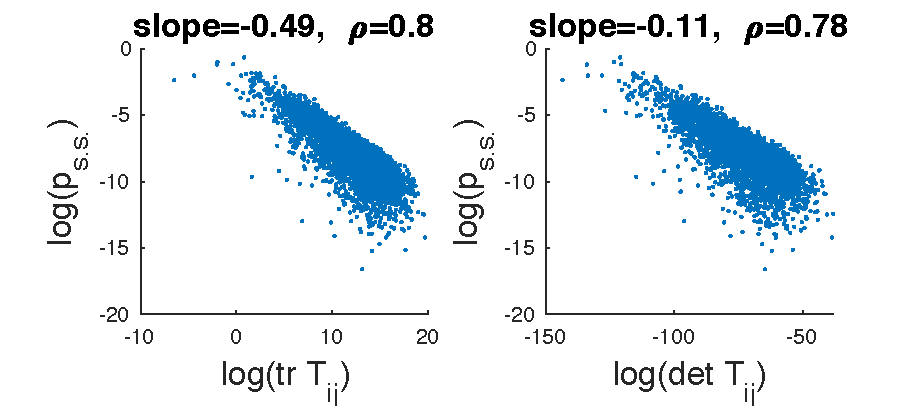
\includegraphics[width=0.5\textwidth]{randForce4D_p4.pdf}
	\caption{Numerical results for motion in 4D random force field, per eq.\ref{eq:randForce}. Effective temperature tensor here $ T_{ij}(x) \equiv F_i(x)F_j(x) $. Regression slope and correlation coefficient are labeled above. \label{fig:randForce}}
\end{figure}

The first thing we note from these results is that both trace and determinant here are similarly well-correlated with $ p_{s.s.} $. We also note that $ p_{s.s.}(x) $ is no longer inverse linear with the trace, as it was in section \ref{app:randDiff}, but now $ p_{s.s.}(x) \sim 1/\sqrt{\tr\[T_{ij}(x)\]} $. This could be understood by seeing that in 1D, the Fokker-Planck dynamics $\dot{p}= \partial_x(F(x)\,p(x)) $ are stationary when $ p(x) \propto 1/F(x) = 1/\sqrt{T(x)} $, for our definition of effective temperature. 

Finally, as in section \ref{app:randDiff}, we can break this correlation by introducing fine-tuned patterns into the force-field. E.g., enhancing the force field along a closed ring, similar as was done for fig. \ref{fig:randDiff2D_br}, produces qualitatively the same sort of results as shown in that figure. 

\subsection{Random discrete map}

For periodically driven systems, as some of our experiments with Smarticles, it may be useful to view the system stroboscopically, making the effective dynamics discrete in time. We can generally express this as:
\begin{align}
x_i(t+1)=f_i(\vec{x}(t)) + \sqrt{2\,T}\,\xi_i
\end{align}
This then gives the probability evolution, which can be expressed in terms of a transfer matrix: 
%\begin{align*}
%p_{t+1}(\vec{y}) =\frac{1}{\sqrt{4\pi T}} \int d^d x \; p_{t}(\vec{x})\,\e{- \frac{1}{4T}\(y_i - f_i(\vec{x})\)^2}
%\end{align*}
\begin{align*}
&p_{t+1}(\vec{y})= \int d^d \vec{x} \;\mathcal{T}(\vec{y},\vec{x})\; p_{t}(\vec{x})\\
&\mathcal{T}(\vec{y},\vec{x}) = \frac{1}{\sqrt{4\pi T}} \; \exp{- \frac{1}{4T}\(y_i - f_i(\vec{x})\)^2}
\end{align*}
The steady-state $ p_{s.s.} $ is thus the dominant eigenvector of $ \mathcal{T}(\vec{y},\vec{x}) $ (with the largest eigenvalue, $ =1 $).

This gives yet another qualitatively distinct class of random dynamics we can study:

%\nocite{*}
\bibliographystyle{unsrt}
%\bibliography{../_data/14654301E131WECPZ6ZSATT3H7YHJ7G6D2E8/default_files/non-equilibSM}
\bibliography{/Users/pchvykov/Documents/GoogleDrive/MIT/RESEARCH/_data/14654301E131WECPZ6ZSATT3H7YHJ7G6D2E8/default_files/non-equilibSM.bib}

\end{document}
